\chapter{Introduction}
\label{chap:intro}

%This is the first chapter.  Here is an example citation:
%\citet{rountree98}.

%%%%%%%%%%%%%%%%%%%%%%%%%%
%% meta-text / overview %%
%%%%%%%%%%%%%%%%%%%%%%%%%%

The thesis presents research into genetic interactions based on genomics data and bioinformatics approaches. Here we introduce the recent developments in genomics and Bioinformatics, particularly in their applications to cancer research. Synthetic lethal interactions are a long standing area of interest to genetics in both model organisms and cancer biology. A bioinformatics approach to synthetic lethal interactions enables much wider exploration of the potential inter-connected nature than previous candidate-based approaches. An alternative approach is experimental screening which will be presented and contrasted with bioinformatics approaches in more detail in the literature review chapter. We outline some of the reasons why these interactions are of interest in fundamental and translational biology but we must first define these and similar interactions. A particularly novel application of synthetic lethal interactions is design of treatments with specificity against loss of function mutations in tumour suppressor genes. We focus on E-cadherin (encoded by \textit{CDH1} as a prime example of this and as such briefly review the role of this gene in cellular and cancer biology.   


%%%%%%%%%%%%%%%%%%%%%%%%%%%%%%%%%%%%%%%%%%%%%%%%%%%%%%%%%%%%%%%%%%%%%%%%%%%
%%%%%%%%%%%%%%%%%%%%%%%%%%%%%%%%%%%%%%%%%%%%%%%%%%%%%%%%%%%%%%%%%%%%%%%%%%%

\section{Cancer Research in the Post-Genomic Era}

Genomics technologies have the potential to vastly impact upon various areas including health and cancer medicine. Considering the progress in recent genomics research, it could soon impact greatly upon clinical and wider applications of genetics either directly or by enabling more focused genetics research from candidates selected from genomics or bioinformatics analysis. The completion of the draft Human Genome marks a major accomplishment in genetics research and raises new challenges to utilise this genomic scale information effectively. Technologies in this area have rapidly developed since and many global large-scale projects have to expanded upon the human genome, to populations, to cancers, and to deeper functional understanding. However, impact on the clinic has been slower than initially anticipated following the completion of the ``draft'' genome with genomics technologies yet to become widely adopted in healthcare and oncology. Here we outline the genomics technologies and bioinformatics approaches which have led to availability of genomics data and techiques used in this thesis and potential for applications in cancer research or the clinic in the future. 

\subsection{The Human Genome Revolution}
The advent of the Human Genome sequence has transformed genetics research \citep{Lander2001}. Systematic, unbiased studies across all of the genes in the genome are viable in unprecedented ways. The successful undertaking of such an international scientific megaproject has set an example for numerous initiatives to follow, including many genomics investigations expanding to species, to the functional, or to the population level. These projects serve are excellent resource for genetics research globally, particularly for cancers where it has been widely applied to different tissues across molecular profiles. Genome sequencing technologies continue to improve, drop in price, and become feasible in more research and for clinical applications.

\subsubsection{The First Human Genome Sequence}
The first human genome is a good example of a large-scale genomics project for it's success as an international collaboration and releasing their data as a resource for the wider scientific community. This particular project generated significant public interest due to it being a landmark achievement, the first of it's scale, and some controversial findings. Namely, the number of genes discovered (particularly those specific to vertbrates) was much lower than most estimates of a genome of it's size and the number of repetious transposon elements was very high. Even the figure of 30-40,000 genes given by the original publication is now widely viewed as an overestimate. 

Accounting for the ``complexity'' encoded by the human genome with so few genes has led to investigations into the molecular function, expression profile, and population variation. When publishing the genome, the author's themselves concede that genomic information alone is not biological understanding and that there is much that remains to be done, with their main goal being to share the raw genome data is available for further inquiry rather than interpreting it themselves. While genomics technologies and genomics projects have flourished since then, the need in turn for systematic means of interpreting data of such scale and for the interdisciplinary expertise to do so has only grown. 

The project originally set out to isolate sections of the genome with labour intensive cloning techniques and individually sequencing DNA with a known locus in the genome by the Sanger methodology scaled up with the capillary sequencing approach. However it became apparent that this would take an incredibly long time and the project shifted to the ``shotgun'' sequencing approach: cutting the genome into many small sections and reconstructing their locus by aligning them by overlapping sections after the sequencing was performed. While sequencing technologies have changed since this project, this paradigm shift in sequencing at the genome-scale stands, with the ``shotgun'' approach being the norm for most sequencing. This represents a shift in genome biology from meticulously tracing the cloned DNA segments to relying on computational approaches to handle the data afterwards, to either assemble genomes \textit{de novo} or map DNA segments to a known reference sequence. This approach was largely successful with the majority (80\%) of the genome being sequenced over 15 months, a relatively short period in the project which began a decade before the announcement of the draft sequence (covering 94\% of the genome). However, it has some shortcomings including handling the repetious regions of a genome.

While some follow-up work has been performed to improve the quality of this sequence, map the distance between contiguous sequences, and ``close the gaps'', repetious regions including the central (centromere) and peripheral (telomere) parts of the chromosomes remains to be mapped. This remains a challenge in modern genomics but for most purposes, the non-repetious aspects of the genome amenable to ``shotgun'' sequencing are sufficient to study the regions of functional importance (such as genes) and of variation between individuals. For this reason nucleotide variation has largely superceeded repetious elements in studies of genetic variability and are used far more widely than structural variants. Genomes continue to be published with incomplete assembles (and accepted to be completed) if the contigs are large enough to be useful for most intents and purposes, particularly if the unknown sequences between contiguous sequences are known. As such, physical distance (length in base-pairs) has largely superceeded genetic distances based on breeding and reference genomes are widely used to faciltate genetics experiments and for wider genomics applications such as mapping genetic variants or expressed genes. Further resources have been developed to enable access to the human genome data such as the ``genome browsers'' provided online by the National Centre for Biotechnology Information (NCBI), University of California Santa Cruz (UCSC), and Emsembl jointly hosted by the European Bioinformatics Institute and the Sanger Institute. 

The ``hierarchical shotgun'' sequence approach was only adopted later in the public Human Genome Project, upon larger fragments already cloned and mapped to particular regions. However, the ``whole genome shotgun'' approach was pioneered by a competing private genome project completed shortly afterwards by Celera Genomics, demonstrating the power and speed of the shotgun approach by sequencing 27 million reads of the entire 2.91Gbp human genome (5.11x coverage) in only 9-months \citep{Venter2001}). Assembly was assisted with the 2.9x coverage public genome data, reduced to raw shotgun reads to reomve cloning bias. While, repetious sequences remained an issue for this project, more than 90\% of the genome was able to be assembled into 100kbp scaffolds and 26,588 protein coding genes were identified, closer to the current consensus for the number of genes in the human genome. This project in particular emphasised the value of computational assembly methods in handling a large number of reads, reducing the time and cost of sequencing, and established the shotgun approach for wider adoption with more recent sequencing technologies with shorter reads.

\subsubsection{Expectations of Genomics}
The human genome attracted a high public profile, particularly with the idea of ``junk DNA'', an unexpectedly large proportion of the genome  which did not appear to be functional. This DNA not encoding genes has since been found to be rich in other functional elements, including microRNA, long non-coding RNA, and regulatory elements such as sites of epigenetic modifications. Genomics has stimulated investigations into many of these previously largely explored areas of functional genetics and thus been of immense value in genetics research, attracting high expectations for further applications. Genomics research has become anticipated for it's potential for widespread applications in healthcare, agriculture, ecology, conservation, and evolutionary biology.

An area of particularly high interest for the clinical impact of genomics is oncology, with potential application across cancer diagnostics, prognosis, management, and developing treatment. Cancers are diseases characterised by uncontrolled cell growth, often driven by genetic mutation or dyregulated gene expression. However, as with many areas of genomics, direct impact of genomics on the clinic has been limited compared to initial expectations following the publication of the human genome and compared with widespread adoption in cancer research. At the time of the genome announcement, it was expected that genomics would become widespread in the clinic and some popular science writers even humoured the idea of ``home genomics'', analogous to how personal computing became adopted by the public. This was largely intended to be for healthcare applications.

Despite significant advances in genomics technologies, including an unprecedented decrease in costs, the most immediate benefit of genomics to patients is indirect usage of the technologies to identify specific biomarkers and drugs to become adopted into clinical practice: diagnostic testing and pharmacological treatment. Clinical adoption of genomics directly raises far more difficult translational challenges. A key issue is ensuring comparable reliability to current genotyping, gene expression, and molecular pathology based on technologies such as polymerase chain reaction (PCR), Sanger Sequencing, or antibody staining. The debatable issue of incidental findings much also be addressed: that is, how to handle or report the additional genetic data gathered from a genome other than that intended to be tested for, such as variants with unknown, potential, or even established malignant implications for the health of the patient.

Along with the overhead costs of genomics being prohibitive to personal usage, the computational demands and genetics expertise required to assemble and interpret a genome have made genomics still largely used for research purposes by institutions. However, some companies are offering direct-to-consumer genetics testing, pushing for public awareness of genetic risks, testing of outwardly healthy people, and preventative medicine. Due to ethical and legal concerns, companies (such as 23andMe) offering genetic testing directly to consumers without clinical consultation have been restricted to reporting on traits for interest and ancestry rather than for healthcare.

\subsection{Technologies to Enable Genetics Research}
\subsubsection{DNA Sequencing and Genotyping Technologies}
Genotyping was once commonly performed on variable regions of the genome with restriction fragment length polymorphisms (RFLP) or repetious microsatellite regions. These exploited sequence variation at target sites of restriction enzymes or measured the length of repetious regions, using polymorase chain reaction (PCR), restriction enzymes, and gel electrophoresis to measure DNA genotypes at particular sites. This is laborious and limited to well cahracterised variable regions of the genome, generally genes or nearby marker regions. 

The Sanger (dideoxy) chain termination method enabled DNA sequencing and genotyping at a wider scale than previously possible. This quickly became more widely adopted  over the Maxam-Gillert sequencing by degradation method develop around the same time due to the technique being less technically difficult and requiring less radioactive and toxic reactants, which have since been replaced by flourescent dyes. Another advantage of the Sanger methodology is the relatively long read length (particularly compared to early versions of more recent technologies), with read lengths of 500-700 base pairs accurately sequenced in most applications, usually following targeted amplification with PCR. Sanger sequencing by gel electrophoresis takes around 6-8 hours and has been further refined with the ``capillary'' approach to 1-3 hours and requiring less input DNA and reactants. The capillary approach has been scaled up to run in parallel from a 96 well plate, at 166 kilobases per hour. The 96 well parallel capillary method was one of the main innovations which made the first Human Genome Project feasible and was used throughout. Due to the quality of the Sanger sequence reads and low cost, it is still widely used in smaller scale applications, clinical testing, and as a ``gold standard'' to validate the findings of newer approaches.


\subsubsection{Microarrays and Quantitative Technologies}
Real-time or quantitative PCR (pPCR) is another adaptation of genetic technologies to quantitatively study nucleic acids, often reverse transcribed ``cDNA'' or messenger ``mRNA'' to measure (relative) gene expression or abundance. While numerous quality control measures are required to correctly interpret a qPCR experiment, these have similarly become widely adopted as are still used for smaller scale experiments and as a ``gold standard'' for measuring gene expression. This also represents a shift in the application of PCR and sequencing technology, where the primary interest is quantifying the amount of input material (by the rate of amplification to a certain level) rather than the qualitative nature of the sequence itself. The more recent technologies of microarrays and RNA-Seq have similarly embraced this application to quantify DNA copy number, RNA expression, and DNA methylation levels. Due to results of comparable or arguably better quality from these newer technologies this ``gold standard'' status has started to come under scrutiny.

Microarrays represent a truly high-throughput molecular technique, reducing the cost, time, and labour required to study molecular factors such as genotype, expression, or methylation across many genes, making it feasible to do so over a statistically meaningful number of samples. Microarrays are manufactured with probes which measure binding of particular nucleotide sequences to either quantitatively detect the presence of a sequence such as a single nucleotide polymorphism (SNP) or quantify for DNA copy number, heterozygousity, expression (cDNA), or methylation (bisulfite treated DNA) purposes. Microarray technologies have popularised ``genome scale'' studies of genetic variation and expression.

In addition to being more versatile and higher-throughput than PCR based techniques, microarrays are considered cost-effective, particularly when scaled up to large number of probes. They are also available with established gene panels or customised probes from a number of commercial manufacturers. These remained popular during the introduction of newer technologies due to reliability and this relatively lower cost, especially in large-scale projects involving many samples. However, microarrays have issues with signal-to-noise ratio with both sensitivity to low nucelic acid abundance and ``saturation'' of probes at high abundance and require more starting material than qPCR. Thus qPCR is still used for many small gene panel studies.

A recently developed alternative to these approaches for gene expression is the ``nanoString'' technology which also samples a selected panel of genes. However, it lacks the scale of microarrays, being effectively limited to 800 probes. This technology differs by giving an absolute measure of the number of transcripts rather than relative measures between genes within a sample, with the manufacturers claiming a higher accuracy. While promising for studies of known genes, such as biological pathways and cancer genes, this technology has not been widely adopted due to higher cost to alternatives and higher-throughput technologies without bias to known genes being feasible. A similar refinement to the qPCR approach, ``droplet'' or ``digital'' PCR also offers to produce absolute measures of transcript abundance. These technologies may become more widely adopted for candidate gene panel research studies and clinical testing with higher data quality as the cost becomes less of an issue. However, the higher throughout of microarray technologies enables a more unbiased approach to test a large number of genes for differential expression for example.

\subsubsection{Massively Parallel ``Next Generation'' Sequencing Technologies}
Similar to microarrays, the introduction massively parallel sequencing technologies have further expanded the availability of high-throughput molecular studies to researchers, with corresponding availability of genomics data from these studies. This ``Next-Generation Sequencing'' (NGS) expands not only gene expression studies (compared to microarrays) but extends to genome sequencing \textit{de novo} for previously unknown genome and transcriptome sequences at an unprecedented scale. This has been a particularly important technological revolution in genomics, as the cost and time of genome sequencing has dropped dramatically and enabled sequencing projects of far more samples and applications beyond the Human Genome Project. Particularly, when dealing with variants in a species with an existing reference sequence such as humans, where the computational cost of mapping to a reference over a genome assembly. However, the cost of sequencing (RNA-Seq) for gene expression or DNA methylation studies is still considerably higher than a microarray study (limiting feasible sample sizes).

Compared with arrays, NGS studies have additional challenges, particularly with large data and compute requirements to handle the raw output data. Compared the the established methods to analyse microarray data, handling NGS data can be more technically difficult. While methods developed for analysing microarray data can be repurposed for sequence analysis in many cases, more bioinformatics expertise is required particularly to handle the raw read data and changing approaches for various changes in sequencing technologies. One of the main computational challenges is the assembly reads or mapping to a reference genome due to the inherently small reads of most NGS technologies compared to the Sanger methodology. Furthermore, there are fewer software releases and best practices established specifically RNA-Seq data, thus many analyses are still conducted with customised analysis approaches and command-line tools. Compared to existing graphical tools or pipelines for microarray analysis, this is a more active technology for bioinformatics research with many applications of genomics data have yet to be explored.

However, there are also additional challenges arising from using data generated from such a recent innovation. This includes ethical issues such as the ongoing debate on how to handle the ``incidental findings'' which may arise from sequencing on such vast scale, particularly with regard to whether NGS technologies are suitable for clinical use and ``variants of unknown significance'', those with undetermined or contested health implications. The methodology itself also has some challenges with the sample preparation, requiring a relatively high quantity of input material and ``contamination'' with over abundant ribosomal rRNA taking up the majority of the sequencing if not purified correctly. This abundance of rRNA is a particularly important issue in RNA experiments in Eukaryotes where it is commonplace target the mRNA by binding to the poly-A tail (RNA-Seq) or 5' cap (CAGE-Seq). However, this has the potential to exclude microRNAs (miRNA) and long non-coding RNAs (lncRNA) of interest unless the sample is prepared specifically to study these. Similarly capturing a subsection of the genome for an ``exome'' or reduced representation bisulfite sequencing (RRBS), focuses on sequencing DNA sequences and methylation levels of CpG sites near known genes to reduce cost, noise, and incidental findings.

In many cases, the benefits of NGS technologies over microarrays still outwiegh the additional cost. NGS is highly adaptable to different applications: DNA sequencing (whole genome or exome), DNA methylation (bisulfite-Seq), RNA-Seq, miRNAs, lncRNA, or chromatin immunopreciptation (CHIP-Seq). NGS scales to all genes and beyond for these molecular applications without having to design new probes as required for a microarray. Thus NGS technologies are not limited to genes already characterised sequence or functions, do not need to be updated with new probes for each genome annotation release, and do not require a reference genome at all for new species. A ``transcriptome'' can be assembled \textit{de novo} for an expression study in any organism.

NGS technologies also have the advantage of greater potential accuracy and sensitivity than microarrays, depending on the sequencing depth or ``coverage'', theoretically sensitive down to the exact number of molecules for each transcript. NGS experiments are regarded as ``reproducible'' with no need for technicals replicates, although these are still performed for a subset of samples in many projects for quality assurance purposes. NGS has a wider dynamic range than microarrays: able to detect SNPS, indels (frameshifts), and splice variants in addition to quantifying DNA copy number or transcript abundance.

Applying NGS technologies varies in cost depending on the platform but is generally substantially more the costly than a microarray experiment for gene expression, limiting the number of sample sizes feasible in many studies.  However, many NGS platforms now support barcoding to label samples and ``multiplex'' their sequencing to perform several samples at once to reduce time and cost of reagents with a sacrifice of read depth. In many cases, this approach is sufficient to compare the expression across many samples and bioinformatics methods are able to correct for varied read depth between samples. Furthermore, refinements of NGS sequencing technologies, the economies of scale, and emerging sequencing technologies have the potential to further reduce the cost of sequencing to the point where it may become feasible for widespread clincal application.  

There is ongoing technology in development to overcome the various drawbacks to established NGS technologies. These emerging technologies, sometimes called ``3 generation'' sequencing aim to introduce radically different approaches to sequencing with distinct advantages. Long reads are the focus of several technologies, accuracy and read length of NGS platforms has improved over time but it is still difficult to assemble or map highly repetious sequences. Another refinement is the sequencing of single molecules in real time, with the potential benefits of low input material and studying 3D structure of nucleic acids. Many of these technologies focus on improving the quality and accuracy of sequences, with higher throughput, read depth, more accurate methodology, avoiding PCR bias or sequencing RNA directly for quantitative studies. Another benefit to highly sensitive sequencing platforms is the potential application in forensic, ancient DNA, and single cell samples where the amount or quality of nucelic acids is low. Single cell applications are of particular interest in cancer research due to the heterogeneity of cells within tumours and their role in diagnostics or drug resistance.

\paragraph{Established Sequencing Technologies}

454 sequencing (acquired by Roche) commercially released from 2005 to 2013 was the first NGS technology, generating a vast 1 million reads per day or 400-600Mbp in a 10 hour run. This technology used the ``pyrosequencing'' method of sequencing by synthesis, detecting phosphates released when a compatible nucleotide reacts and extends the DNA synthesis of a complementary strand. This technology popularised NGS with the first complete genome from a single individual (James Watson, 2007) and the Neanderthal ancient DNA studies (Svaante Paabo, 2006 \& 2009). While this technology was capable of reads up to 1kb, reads of 400-500bp were more typical and the error rate was higher for sequences of the same base consecutively. This is still relatively long reads for an NGS technology but it has been discontinued due to competing short read technologies being more cost-effective with lower running costs.

SOLiD sequencing (acquired by Life Technologies) released in 2006 employs a vastly different approach to NGS, using labelled dinucleotide pairs for ``sequencing by ligation'' to produce a highly accurate sequence (99.94\%) with built-in error correction by sequencing two reading frames and is unaffected by consecutive bases. This technology is also high-throughput, producing 1200-1400 million reads (66-120Gbp) in a 7-14 day run. However, SOLiD sequencing does not cope well with palindromic sequences and SOLiD reads are very short only 35bp, making it more difficult to assemble them.

Illumina sequencing (developed by Solexa and later acquired by Illumina) was also released in 2006. It utilises reversible terminating dyes to sequence by synthesis with a lower accuracy (98\%) and read lengths of 150-250bp. Illumina more than makes up for relatively short reads (along with improving the read length of the technology) and low accuracy with high-throughput and cost effectiveness, with a Hi-Seq 2500 platform producing up to 3 billion reads (600Gbp) in a 3-10 days run. Illumina has further reduced the cost of sequencing with the economies of scale with the HiSeq 10X claiming to produce a human genome for less than US\$1000, the first platform to achieve this long-standing goal in genomics. The high-throughput of Illumina sequencing also makes deep sequencing for high coverage, high quality consensus reads, and sensitive RNA-Seq experiments feasible. Illumina sequencing now has a dominating market share of the NGS technologies.

\paragraph{Emerging Sequencing Technologies}

Ion Torrent (also acquired by Life Technologies) released in 2010 employs ``sequencing by synthesis'' but in a drastically different way with ion semiconductor sequencing, detecting $H^+$ ions released when bases during DNA synthesis. Without the use of optical detection, the Ion Torrent system is compact offering rapid, cost-effective sequencing with the potential to scale with the future development of silicon semiconductors with have historically doubled in density every 2 years (Moore's Law). It is capable of reads of 100-200bp in only an hour (as fast as 4 seconds per base) and up to 400bp in a 2 hour run with an accuracy of 99.6\% (dropping to 98\% for consecutive sequences of 5 bases). While fast, cost effective, and accurate, Ion Torrent has short reads and modest throughput (depending on the platform 100Mbp to 32Gbp) compared to other sequencing technologies.

Pacific Biosciences (PacBio) released the RS and RS II platforms in 2010 and 2011 (now acquired by Roche) to make up for the short reads in NGS technologies with the single molecule real time (SMRT) approach capable of long read lengths, averaging between 2.5-7kb and up to 80kb. The PacBio methology traps each molecule in a zero mode waveguide (ZMW) and sequences it in real time. The RS II has 150,000 ZMW and an output of 500Mbp-1Gbp per SMRT cell (doubling that of the RS), with the capacity to run up to 16 concurrently for 0.5-6 hours. While the single molecule sequencing approach has strengths in sensitivity and potential to detect 3D structures, such as G-quadruplexes, this has the drawback of slowing down the sequencing and reducing the throughput of the platform. Another issue is sequence quality with the raw data as poor as 20-30\%. However, PacBio recommends specific software to assemble as consensus with 99.999\% ($Q_{50}$ for sequences with over 20x coverage, regardless of sequence repeats or GC composition. Despite concerns over data quality and higher cost than other approaches, the long reads are appealing for genome assembly and in many genome studies combine PacBio reads with more accurate short read technologies. However, due to the poor separate quality of reads this technology may not be appropriate for RNA-Seq studies, while it does have the potential for high sensitivity and detecting alternative splicing were it be improved. PacBio has recently released the Sequel (2016) system, increasing the throughput of the SMRT Cells 7x to 1 million ZMW holes. 

Nanopore sequencing is another technology capable of long reads in real time and direct single molecule sequencing, avoiding amplification bias, detecting modified bases and directly sequencing RNA molecules. This also reduces laboratory preparation times. Nanopores work by measuring the ion current through a pore in a electrically insulating membrane as a nucleic moves through it. Oxford Nanopore has been developing this technology since 2005, launching the MinION in 2014 which employs biological nanopores: a transmembrane protein through which DNA or RNA passes, blocking ion current differently for each base. Each pore sequences in real time, capable of sequencing 450bp per second. However, the are quality issues with each individual read with quality estimates varying between 87-98\%, with improvements to the quality of detection accounting for significant delays in the release of this technology. The MinION makes up for the is a capacity for extremely long reads, averaging 5.4kbp (Hayden, 2014) up to a maximum of 200Kbp and being a portable platform with very few overhead costs. While the MinION is limited in scale with only one flow cell of 512 pores (5-10Gbp), the PromethION being released in early access in 2016 scales this technology with flow cells of 3000 pores and the capacity to run 48 (up to 4 samples each) in parallel for 144,000 long reads with a versatile, modular system including built-in computing resources. One of the main issues with Oxford Nanopore systems is accuracy, with the manufacturer suggesting the use of consensus sequences for higher accuracy as PacBio does. The main source of this pore accuracy is the width of biological pores resulting in several bases being in the pore at any one time, inferring the sequence from the ion currents of each respective combination of bases and distinguishing them is a major technical challenge.

Quantum Biosystems in Japan is developing a synthetic nanopore system to address this issue. While the technology is still in development, it has the potential to produce similarly long reads, with a high-throughput, low running cost, and rapid run time. The technical challenges to develop a nanotechnology capable of this are immense but such developments serve as but one of example of how sequencing technologies may continue to improve, becoming more feasible for a wider variety of applications.

%%%%%%%%%%%%%%%%%%%%%%%%%%%%%%%%%%%%%%%%%%%%%%%%%%%%%%%%%%%%%%%%%%%%%%%%%%%%%
%% RNA-Seq focus of this thesis over previous work on TCGA microarray data %%
%%%%%%%%%%%%%%%%%%%%%%%%%%%%%%%%%%%%%%%%%%%%%%%%%%%%%%%%%%%%%%%%%%%%%%%%%%%%%

Due to such benefits of sequencing over previous technologies (and their continued refinement), this thesis has focused on RNA-Seq data in contrast to prior studies on microarray data. RNA-Seq data is widely available as a resource from large-scale cancer genomics projects and methods to make inferences from RNA-Seq experiments could feasibly be applied to many other studies based on these current (or similar future) technologies.

%\subsubsection{The Future of Genomics Research}

\subsubsection{Bioinformatics as an Interdisciplinary Approach to Genomics Data}
Genomics technologies have given rise to data at a scale previously rarely encountered in molecular biology, making inference with conventional techniques difficult. Computational, Mathematical, and Statistical skills are required to handle this data effectively, in addition to biological background to frame and interpret research questions. Drawing upon these disciplines to handle biological data has become the field of ``Bioinformatics", focusing specifically on making inferences from genomics and high-throughput molecular data or developing the tools to do so. This contrasts with the existing fields of ''theoretical`` or ''computational biology`` which existed prior to genomics data, focusing on modelling and simulating aspects of biology without necessarily addressing the genomics data or detecting the phenomena in nature, extending beyond to genetics to cell modelling, neuroscience, cancer development, ecology, and evolution.

In practice, many researchers identify with both fields or draw upon the findings and methods of the other field. This thesis uses many approaches in bioinformatics to biological research questions and established Mathematical and Bioinformatics reseources.

Gene expression analysis is the focus of many bioinformatics research groups, drawing upon statistical approaches to appropriately handle microarray and RNA-Seq data along with making biological inferences from a large number of statistical tests. This presents various challenges from normalising sample data and accounting for batch effects to developing or applying statistical tests tailored to biological hypotheses and testing them at a genome-wide scale, generally across thousands of genes. There are numerous approaches for dealing with these challenges, some of which will be described in the methods chapter (2).

\subsection{Follow-up Large-Scale Genomics Projects}
A number of projects have attempted to follow up on the human genome project to varying degrees of success. The genomes have since been sequenced for a variety of model organisms, organisms of importance in health, agriculture, metagenomics of microorganisms (microbiome), ecology and conservation. The International HapMap Project, 1000 Genomes Project, and the 100K Genome Project aim to gather genetic variation data across human populations, along with gathering clinical and environmental variables for health and disease association studies. Whereas the ENCODE, ModENCODE, and FANTOM projects aim to characterise the functional aspects of human and model organism genomics. ENCODE in particular has attracted much criticism for over-inflated claims of DNA functionality. A notable finding of the ENCODE projects is that a high number of DNA sites bind to proteins or are transcribed into RNAs. However, these are not necessarily of functional importance. Conversely, the FANTOM projects approach this problem by focusing on expressed mRNAs, microRNAs, and epigenetic marks in each tissue or cell type. An area of recent interest are the long non-coding RNAs, the focus of FANTOM6, the next phase of the project amenable to the CAGE-Seq technologies developed in prior FANTOM projects.

Other genomics databases have focused on faciltating distribution of genomic data generated by researchers, rather than generating it themselves. Genbank (NCBI) in the US, EMBL in Europe, and the DDBJ (NIG) in Japan do so by serving as repositories of DNA sequence data. GEO, arrayExpress, and caArray serve a similar purpose as a resource for gene expression datasets. These serve as a resource to support ongoing research to ulitise data for genes of interest to particular research groups and further to make inferences based on larger datasets than accessible to any individual laboratory.

These resources cover not only DNA sequence across the genome but also molecular profiles of other factors by adapting genomic sequencing or other high throughput technologies. Reverse transcribed RNAs are a common such adaptation, employing RNA-Seq to the transcriptome. This is ulitised to be quantify the levels of RNA and identify which regions of DNA are expressed. Similar bisulfite treatment converts cytosine residues to uracil (sequenced as thymidine), sparing methylated cytosine enabling it to be distinguished with bisulfite-Seq for high-throughput detection of the notable epigenetic mark and generating an epigenome. High-throughput gel and mass spectrometry techniques have been employed to proteins and metabolites to generate the proteome and metabolome respectively. In this way, so called ``omics'' profiles across a wide range of biomolecules in a cell are produced in many experimental laboratories. SUch genomics technologies have since been applied to single cell isolates and to detect traces of foetal or tumour molecules in blood or urine.

Similarly, international projects and consortiums have begun to release data gathered using common agreed upon protocols in laboratories across the world, often hosting public databases of these themselves, publishing their own investigations into the datasets as they are released, or offering basic searches and analytics of the data via a web portal. These databases include many of the genomics projects discussed above and the cancer-specific projects discussed below. In many ways, the quality, consistency, and accessibility of these international projects has become more appealing than accessing smaller studies, particularly for gene expression datasets where the more recent, larger projects have switched from microarray to RNA-Seq technologies. This distinction will also be discussed later.

\subsection{Cancer Genomes}
It's importance in the future of cancer research was noticed, even in the early days of genomics (Dickson, 1999). The Cancer Genome Project (CGP) based at Wellcome Trust Sanger Institute in the UK were among the first to launch investigations into cancer after the publication of the Human Genome, using this genome sequence, consensus across the cancer reserach literature, and sequencing the genes of cancers themselves. Initially, the Sanger Institute set out to sequence 20 genes across 378 samples while the Human Genome project was still ongoing (Collins and Baker, 2007), optimising sequencing and computation infrastructure for a larger project while doing so. The main aim of the Cancer Genome Project was to discover ``cancer genes'', those frequently mutated in cancers by comparing the genes of cancer and normal tissue samples, both ``oncogenes'' and ``tumour suppressors'' which are activated and inactivated respectively in cancers. This project is ongoing and the UK continues to be involved in international sequencing initiatives and those focused on particular tissue types.

The Sanger Institute also hosts the Catalogue of Somatic Mutations in Cancer (COSMIC), a database and website of cancer genes. This launch with 66,634 samples and 10,647 mutations from initial investigations into \textit{BRAF}, HRAS, \textit{KRAS}2, and NRAS (Bamford, 2004). It has since expanded to include 1,257,487 samples with 4,175,8787 gene mutations curated from 23,870 publications, including 29,112 whole genomes (Release v79 (23/08/2016 \url{http://cancer.sanger.ac.uk/cosmic}). This database now also identifies cancer genes from DNA copy number, differential gene expression and differential DNA methylation.

\subsubsection{The Cancer Genome Atlas Project}
Based in the US, the Cancer Genome Atlas (TCGA) project was established in 2005, a combined effort of the National Cancer Institute (NCI) and the National Human Genome Research Institute (NHGRI) of the National Institutes of Health (NIH). They first set out to demonstrate the pilot project on brain (2008), ovarian (2011), and lung (2012) cancers. In 2009, the project expanded aiming to analyse 500 samples each for 20-25 tumour tissue types. They have since exceeded that goal, with data available for 33 cancer types including 10 ``rare'' cancers, a total of over 10,000 samples.

The TCGA projects set out to generate a molecular ``profile'' of the tumour (and some matched normal tissue) samples: the genotype, somatic mutations, gene expression, DNA copy number, and RNA methylation levels. While these were originally performed largely with microarray technologies, exome and RNA-Seq has been since adopted and performed for many TCGA samples, with whole genomes being performed for some samples. Data which cannot be used to identify the patients (such as somatic mutation, expression, methylation, and various clincal factors) are publicly available.

\subsubsection{The International Cancer Genome Consortium}
TCGA and the Cancer Genome project in the UK are part of a larger International Cancer Genome Consortium (ICGC), now a concerted effort across 16 countries to sequence the genome, transcriptome, and epigenome of 50 tumour types from over 25,000 samples total. With some redundancy the following countries are profiling various tumour types: USA (including TCGA), China (16), France (10), Australia (4), South Korea (4), the UK (4), Germany (4), Canada (3), Japan (3), Mexico (3 in collaboration with the US), Singapore (2),  Brazil, India, Italy, Saudi Arabia, and Spain. This is inherently international and several projects are collaborations, such as between the USA and Mexico, Australia and Canada, Singapore and Japan, along with the UK and France representing the European Union. In order to avoid competing the existing TCGA projects, some countries focus on a particular cancer they have health interest: Australia (melanoma), Brazil (melanoma), India (oral), Saudi Arabia (thyroid), and Spain (CML). Others focus on a particular tissue subtype with poor prognosis: The UK (triple negative or Her2$+$ breast cancer), France (clear cell kidney), Australia and Canada (ductal Pancreas). Another approach is to focus on rare or child cancers: Canada, Italy, France, Germany, Japan and Singapore, and the US (TARGET project). Particularly countries in Asia (China, Japan, Singapore, and South Korea883 samples) have emphasised the value of adding tumour data from non-Western countries or non-European populations in addition the data from Europe and the TCGA in the US. Data from 9 of these countries is already available on the ICGC website with the project ongoing.

\subsubsection{Sub-population and Cell Line projects}
Similarly, the San Antonio Cancer 1000 Genome Project also focuses on the genomics and clinical data of their local population. There is a growing emphasis on ensuring that genomics findings are applicable to populations beyond studies in European cohorts, such as the inclusion of Hispanic and African American individuals in genomics studies in the US, dedicated genomics projects on Asian populations from China, India, Japan, and Singapore being included as part of ICGC, and recent studies into cancer, healthcare, or genomics of indigenous populations such as New Zealand  M\={a}ori, Australian Aboriginal, Torres Strait Islanders, Hawaiian, and Native American populations. 

Another more specific project is the Molecular Taxonomy of Breast Cancer International Consortium (METABRIC) a joint project between Canada and the UK focusing particularly on breast cancer. The METABRIC project gathered the genome and transcriptome of 2,433 samples to identify driver mutations and breast cancer subtypes. Other projects have extended the genomics technologies to profile cancer cell lines used in research, including the Cancer Cell Line Encyclopaedia (CCLE) and the COSMIC Cell Lines projects. The CCLE run by the Broad Institute and Novartis has analysed 883 cell line samples including DNA copy number, array expression, mutaions, and  drug response data. The COSMIC project aims to profile 1000 cell lines by exome, copy number, expression (RNASeq), DNA methylation.

These projects represent a massive ongoing global effort to understand cancers at the molecular level across the genome and beyond. They serve as a fantastic resource for further analysis, being publicly released, regularly updated, and making sample sizes far higher than feasible in prior microarray studies. The potential of genomics in cancer research is widely recognised as is the value of technological and bioinformatics advances to enable it to continue to do so. 


\subsection{Genomic Cancer Medicine}
There is much anticipation in cancer research for genomics technologies to have a clinical impact in cancer medicine: from diagnosis and prognosis to treatment developments and strategies. These may result either from direct use of genome or RNA-Seq in clinical laboratories or indirectly from biomarkers and treatments developed with research faciltated by genomics. This second strategy is likely to have a more immediate patient benefit due to the cost of genome sequencing, particularly considering adoption in public healthcare systems with a limited budget.  

\subsubsection{Cancer Genes and Driver Mutations}
There are two main categories of ``cancer genes''. Oncogenes are those activated in cancers either by gain of function mutations in proto-oncogenes, amplification of DNA copies, or evelated gene expression. Their normal functions are typically to regulate stem cells or to promote cellular growth and recurrent mutations are typically concentrated to particular gene regions. Conversely, tumour suppressor genes are those inactivated in cancer either by loss of function mutations, deletion of DNA copies, repression of gene expression, or hypermethylation. Their normal functions are typically to regulate cell division, DNA repair, and cell signalling.

Detecting these cancer genes is a major challenge in cancer biology and has been revolutionised by genomic technologies. Recurrent mutations, or DNA copy number variants and differential gene expression or DNA methylation are all indicative or cancer genes which can be detected in genomics data. Important ``driver'' cancer genes are difficult to detect from ``passenger'' mutations due to patient variation, tumour heterogeneity, and genomic instability. However, many cancer genes have been replicated from previous studies or well supported from genomics data. There remains the challenge of translating the identification of cancer genes to patient benefit with characterisation of variants of unknown significance, which mutation or gene expression markers can be used to monitor tumour progression or treament response, and design of therapeutic intervention against many molecular target for which they have yet to be developed or repurposed from other disease to cancers. 

\subsubsection{Personalised or Precision Cancer Medicine}
The notion of using a patient's genome to tailor healthcare to an individual has been appealing since the advent of genomics, popularised with the term ``personalised medicine''. This approach was expected to span from preventative lifestyle advice to effective treaments. Personalised medicine was intended contrast with current strategies of health advice, screening, prognostics, and treaments based on what works well with the majority of the population, highlighting that adverse effects of treaments occur in a significant subpopulation and that many clinical studies are dominated by Western populations of European ancestry and may not generalise to other populations.

While the importance of genomics is still recognised in translational cancer research, it's potential has been emphasised particularly in molecular diagnosis, prognosis, and treaments of patients already presenting with cancers in the clinic rather than preventative medicine. This is in part due to the vast number of variants of unknown clinical significance, the ethical issue of reporting on incidental findings, and the regulatory issues direct-to-consumer genetics companies have encountered offering health risk assessment.

More recently the term ``Genomic medicine'' has been preffered the describe the paradigm of treating cancers by their genomic features, particularly grouping patients by the mutation, expression, or DNA methylation profiles of their cancers. Radical proponents advocate for these molecular subtypes to superceed tissue or cell type specific diagnosis of cancers. However, in practice they are often used in combination, with clinical and pathological factors being informative of prognosis and surgical training specialising by organ system. The related term of ``precision medicine'' also stems from this trend with the rationale to target these molecular subtypes with separate treatment strategies, particularly in developing and applying treaments targeted against a particular mutation specific to cancers. To this end much research in this field is focused on identifying mutations and gene expression signatures amenable to distinguishing cancers, particularly oncogenic driver mutations, and developing treatments against them.

\paragraph{Molecular Diagnostics and Pan-Cancer Medicine}
There is growing support for the use of molecular tools such as mutations or gene expression signatures to diagnose tumour subtypes in replacement or addition to tissue of origin or histology. This is particularly important is breast cancer where several distinct ``intrinsic subtypes'' have been identified from molecular data with differences in malignancy and patient outcome (Parker/Perou). These have been popularised with the idea of ``Pan cancer'' studies such as those conducted by the TCGA and ICGC projects, combining molecular profiles across tissue types. The molecular subtypes could feasibly be included in clinic testing as a panel of biomarkers for diagnostics and prognosis. Such biomarkers also have the potential to monitor drug response or risk of recurrence. This is also raises the need for development of treatments for targeting these molecular subtypes.  

\subsubsection{Targeted Therapeutics and Pharmacogenomics}
Targeted therapies with specificity against a molecular target are emerging as means for precision cancer medicine. While these molecular targets can be tested in laboratory conditions with RNA interference, pharmacological agents are required for treatment in patients. However, identification of molecular targets is also an important step towards novel anti-cancer treatments, followed by validation and drug testing to develop a targeted treatment. This is relatively straight-forward with oncogenic mutations where the recurrent mutant variant or overexpressed gene can be directly inhibited by pharmacological antagonists. The main approaches are structure-aided drug design (based on known protein structures of oncoproteins) or compound screening (for activity against the oncoprotein). Targeting oncogenes with high homology to other genes or tumour suppressor genes lost in cancers is not amenable to direct targeting.

Monoclonal antibodies have been developed against several oncogenes but more affordable small compounds are preferable for their feasibility in public healthcare systems with wider potential for patient benefit. Monoclonal antibodies such as herceptin against \textit{HER2} in breast cancer have been controversial due to their prohibitively high cost. Despite this controversy, targeted therapeutics have been applied against several oncogenes across cancer tissue types with relative sucess in clinical trials, generating considerable interest in wider application of this approach. The main advantage of targeted therapeutics is their specificity in targeting tumour cells, having a wide therapeutic window compared to cytotoxic chemotherapy (prone to severe side effects against healthy rapidly growing tissues). Thus targeted therapeutics can be effective against advanced stage cancers since high doses can be tolerable and could feasibly be applied against early stage cancers or as a chemopreventative in individuals with a high genetic risk of developing cancer. Targeted therapeutics could also feasibly be applied in combination against several molecular targets, with reduced doses of standard chemotherapy and radiation, or with emerging endocrine and immunological treatments.

Pharmacogenomics is another potential application using genomic variants to predict have adverse effects to either conventional treatments or targeted therapies. Patient variation is a clinically important challenge in cancer therapy and anticipating adverse effects, drug resistance, and dosing effectively are all ways in which genomics could facilitate more effective use of existing treatments and inform development of novel treatments against specific molecular targets.

\paragraph{Targeting Oncogenic Driver Mutations}
%\paragraph{Tissue Specificity and Genetics Background Effects}
Oncogene targeted therapies have also been developed with some examples of effective clinical application against cancers. However, they already begun to manifest problems with resistance, recurrence, tissue specificity, and design of inhibitors specific to oncogenic variants rather than proto-oncogene precusors. Targeted anticancer therapeutics can exploit complex interactions to distinguish normal and cancerous cells which may benefit from studies of gene regulation or interaction networks. The unexpected synergy between inhibitors of the oncogenes \textit{BRAF}\textsuperscript{V600E} and \textit{EGFR} in colorectal cancersis an example of such a system (Prahallad2012)

\textit{BRAF} is a serine/threonine kinase gene in the MAP kinase pathway with several oncogenic mutations including the V600E mutation, a driver of some cancers including colorectal, hairy cell leukaemia, lung, and melanoma (Entrez Gene). The epidermal growth factor receptor (\textit{EGFR}) gene detects extracellular ligands including epidermal growth factor (EGF) and  transforming growth factor (TGF$\alpha$). Overexpression of \textit{EGFR} is itself oncogenic in brain, colorectal, and lung cancers (Entrez Gene). Both oncogenes have been explored in some detail as separate drug targets with successful development of drugs acting against \textit{BRAF}\textsuperscript{V600E} in melanoma and drugs against \textit{EGFR} in lungs cancers, however they have limited efficacy separately in colorectal cancer.  

\textit{BRAF}\textsuperscript{V600} mutations are a feasible target for anticancer therapy, occurring in 8\% of all solid tumours including substantial numbers of melanomas, thyroid, and 10-15\% of colorectal cancers (Davies2002). \textit{BRAF} mutant tumours use the MAPK/ERK (extracellular signal-regulated kinase signalling cascade) pathway to induce tumour growth (Dienstmann \& Tabernero 2011). The specific inhibitor vermurafenib is more effective than non-selective MEK downstream targets effective in melanoma cells (Dienstmann \& Tabernero 2011) and is suitable for treatment of \textit{BRAF}\textsuperscript{V600E} mutant melanomas, with success in phase I-III clinical trials and FDA approval (Ravnan \& Matalka 2012). \textit{BRAF} inhibitors have desirable efficacy and toxicity but acquired drug resistance is a serious problem in melanoma, as such biological mechanisms are needed to ensure optimal clinical outcomes (Dienstmann \& Tabernero 2011). \citet{Ravnan2012} suggest combination therapy as a solution to vemurafenib resistance in melanoma.  

Despite successful application of vemurafenib against \textit{BRAF}\textsuperscript{V600E} in melanomas, colorectal cancers with \textit{BRAF}\textsuperscript{V600E} mutations have poor prognosis and lack drug response. \citet{Prahallad2012} used an RNAi kinome screen in the WiDr colon cell line. \textit{EGFR} inhibition is synergistic with vemurafenib aginst \textit{BRAF}\textsuperscript{V600E} in celllines and xenografts. This synergy arises mechanistically from feedback activation of \textit{EGFR} in response to \textit{BRAF} inhibition, consistent with higher \textit{EGFR} expression in colorectal and thyroid cancer cell lines compared to melanoma cell lines and vemurafenib resistance induced from ectopic \textit{EGFR} expression in melanomas. \citet{Corcoran2012} supported this mechanism with transient inhibition of \textit{BRAF}\textsuperscript{V600E} by vemurafenib which induced rapid reactivation of MAPK/ERK signalling via \textit{EGFR} in colorectal cell lines. This did not occur in melanoma cell lines suggesting colorectal tissue-specific regulation of \textit{EGFR} and supporting the use of combined \textit{BRAF}\textsuperscript{V600E} and \textit{EGFR} inhibitors which effectively block MAPK/ERK signalling in cell lines and xenografts. Across these studies, synergy between vemurafenib and \textit{EGFR} inhibitors was replicated for multiple \textit{BRAF} mutant colorectal cell lines with both antibody (cetuximab) and small-molecule drugs (gefitinib and erlotinib) giving a mechanistically derived means to overcome vemurafenib resistance.  

\citet{Sun2014} applied these findings to vemurafenib resistance in \textit{BRAF}\textsuperscript{V600E} melanomas. \textit{EGFR} expression was an adaptive response to \textit{BRAF} or MEK inhibition in \textit{BRAF} mutant biopsies and cell lines. A chromatin regulator RNAi screen on A375 melanoma cell line with low initial \textit{EGFR} expression and selection for vemurafenib resistance which showed that \textit{EGFR} overexpression occurred only after \textit{BRAF} gene silencing and drug selection. \textit{SOX10} was the only gene with multiple shRNAs which induce \textit{EGFR} overexpression and \textit{SOX10} was sufficient \textit{EGFR} expression and TGF$\beta $ signalling. \textit{EGFR} overexpression or TGF$\beta$ exposure cause may cause a slow growth phenotype (oncogene-induced senescence), being only beneficial to melanomas under drug selection. Heterogeneous \textit{SOX10} expression account for variation in selection and vemurafenib resistance in melanoma cell lines. \textit{SOX10} expression and vemurafenib sensitivity are restored when \textit{BRAF} inhibition is removed, supporting a drug holiday approach against drug resistance.  

These have lead to various ongoing clinical trials. Combination treatment of vemurafenib (as a \textit{BRAF} inhibitor) and various FDA approved \textit{EGFR} inhibitors entered phase I clinical trials for treatment of \textit{BRAF}\textsuperscript{V600E} mutant tumours in 2014. Vemurafenib and panitumamab are being trialled in colorectal cancers by the Memorial Sloan Kettering Cancer Center, New York. Combination treatment of vemurafenib, cetuximab (an \textit{EGFR} inhibitor) and irinotecan (a topoisomerase inhibitor) are being trialled in advanced solid cancers by the MD Anderson Cancer Centre, Houston. Combination vemurafenib and erlotinib are being trialled in \textit{BRAF} mutant cancers including colorectal and lung by the Peter MacCallum Cancer Centre, Melbourne.  

\paragraph{ Network Medicine, and Polypharmacology}
Targeted therapeutics have had some success for drug discovery, particularly in anticancer applications, exploiting the molecular networks or designing combination therapies may yield more effective results with a network pharmacology framework (Hopkins 2008). Rational design of drugs selective to a single target has often failed to deliver clinical efficacy. Many existing effective drugs modulate multiple proteins, having been selected for biological effects or clinical outcome rather than molecular targets. Proponents of network biology and polypharmacology (specific binding to multiple targets) recommend to develop drugs with a desired target profile designed for the target topology (Hopkins 2008; Barabasi and Oltvai 2004). Multi-target treatments aim to achieve a clinical outcome through modulation of molecular networks since the genetic robustness of a cell often compensates for loss of a single molecular target.  

While multi-target drugs may be more difficult to design, they are faster to test clinically than drug combinations which are usually required to be tested separately first (Hopkins 2008). Networks have already been exploited to design synthetic lethal treatments for cancer, drug combinations and multi-target drugs to combat resistance to chemotherapy and antibiotics (Hopkins 2008; Barabasi and Oltvai 2004). Nevertheless, further optimisation of timing and dosing of drug combinations may increase efficacy and needs to be explored for combination effects with low efficacy as separate treatments. Low doses and drug holidays are other counter intuitive approaches which may increase clinical efficacy, reduce adverse effects, and reduce drug resistance (Sun2014; Tsai2012).  

A network understanding of a cell has the potential to impact upon drug design and clinical practice, particularly in treatment of cancer and infectious disease. Characterisation of the target system and impact of existing treatments, such as  \textit{BRAF}\textsuperscript{V600E} and \textit{EGFR} inhibitors, enable wider application of the mechanisms for such interventions exploiting genetic interactions or pathways. This could lead to development of more effective treatment interventions for these systems and prediction of similar molecular systems for development of novel drug targets and combinations.  


%%%%%%%%%%%%%%%%%%%%%%%%%%%%%%%%%%%%%%%%%%%%%%%%%%%%%%%%%%%%%%%%%%%%%%%%%%%
%%%%%%%%%%%%%%%%%%%%%%%%%%%%%%%%%%%%%%%%%%%%%%%%%%%%%%%%%%%%%%%%%%%%%%%%%%%

\section{A Synthetic Lethal Approach to Cancer Medicine}

Synthetic lethality has vast potential to improve cancer medicine by expanding application of targeted therapeutics to include inactivation of tumour suppressors and genes that are difficult to target directly. Synthetic lethal interactions are also studied for gene function and drug mode-of-action in model organisms. This section introduces the concept of synthetic lethality as it was originally concieved and how it has been adopted conceptually in cancer research. Detecting these interactions at scale and interpreting them is the focus of this thesis, hence we start with an overview of the concepts involved, initial work on the interaction, and the rationale for applications to cancer. Specific investigations into synthetic lethality in cancer, detection by experimental screening, and prediction by computational analysis will then reviewed.


%Synthetic lethal interactions occur when mutations in two or more non-essential genes lead to inviability or growth defects at a cellular or organism level. These genetic interactions arise from functional redundancy between genes, making them useful as a model for gene function or drug mode-of-action studies, and as an emerging strategy for anti-cancer drug design against loss of function mutations \citep{Boone2007,Kaelin2005}. Any perturbation of synthetic lethal genes including DNA hyper-methylation, gene under-expression, or pharmacological inhibition of protein function can induce cell death, thus enabling studies and screens with RNA interference (RNAi) and chemical agents \citep{Fece2015}.

%Many genes are lost or altered in cancers, so exploiting synthetic lethality could enable targeting a wide range of cancer specific aberrations in gene function or expression, including tumour suppressor defects that are not targeted by conventional drug design strategies \citep{Kaelin2009}. As tumours develop and become genomically unstable, genes lost make them vulnerable to specific killing by inhibition of synthetic lethal genes. Synthetic lethal partners of tumour suppressor genes are therefore cases of `non-oncogene addiction' and `induced essentiality' alluding to similarities with other genetic processes involved in cancers \citep{Fece2015, Luo2009}.


\subsection{Synthetic Lethal Genetic Interactions}
Genetic interactions are a core concept of molecular biology, discovered among earliest investigations of Mendelian genetics, and recieving revived interest with new technologies and potential applications. Biological epistasis is defined as the effect of an allele at one locus may mask the phenotype of another (Bateson \& Mendel 1909). Statistical epistasis is defined as the significant disparity between the observed and expected phenotype of a double mutant, compared to the respective phenotypes of single mutants and the wild-type (Fisher 1919). Fisher's definition lends itself to quantitative traits and more broadly encompasses Synthetic genetic interactions (SGIs). These have become popular for studies in yeast genetics and cancer drug design (Boone2007; Kaelin 2005).


Synthetic genetic interactions are substantial deviations of growth or viability from the expected null mutant phenotype (of an organism or cell) assuming additive (deleterious) effects of the single mutants. In contrast to biological epistasis, this deviation does not necessarily constitute a single mutant phenotype (as shown in Figure \ref{fig:Costanzo2011}). Mose SGIs are more viable than either single mutant or less viable than the expected double mutant. Mutations are ``synergistic'' in negative SGIs with more deviation from the wild-type than expected. Formally, ``synthetic sick'' (SSL) and ``synthetic lethal'' (SL) interactions are negative SGIs giving growth inhibition and inviability respectively. Synthetic lethality in cancer research more broadly describes any negative SGI with specific inhibition of a mutant cell, including SSL interactions. Mutations are ``alleviating'' in positive SGIs with less deviation from the wild-type than expected. For viability, the terms ``synthetic suppression'' (SS) and ``synthetic rescue'' (SR) are positive SGIs giving at least partial restoration of wild-type growth from single mutants with growth impairment and lethal phenotypes respectively. Negative SGIs were markedly more common than positive SGIs in a number of studies in model systems (Tong2004; Boucher \& Jenna 2013). 

\begin{figure}[!ht]
   \centering
   \resizebox{0.75 \textwidth}{!}{
   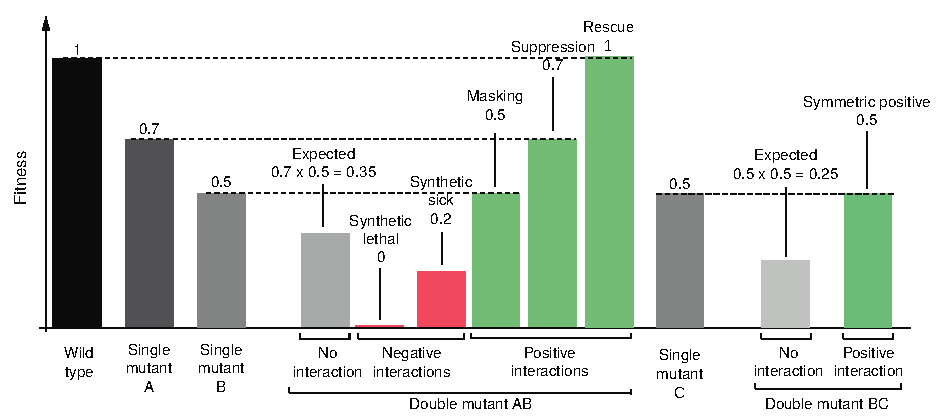
\includegraphics{Costanzo_2011_SL_mega_no_border.pdf}
    }
   \caption[Synthetic genetic interactions]{\textbf{Synthetic genetic interactions.} Impact of various negative and positive SGIs on growth viability fitness in yeast. Adapted from \citep{Costanzo2011}.}
\label{fig:Costanzo2011}
\end{figure}

\subsection{Synthetic Lethal Concepts in Genetics}

Synthetic lethal genes are generally regarded to arise due to functional redundancy. Due to the functional level of SGIs, synthetic lethal genes do not need directly interact, nor be expressed in the same cell or at the same developmental stage: serving related functions is sufficient to affect cell (or organism) viability and be relevant to drug-mode-of-action cancer biology. Combined loss of genes performing an essential or important function in a cell are therefore deleterious. Synthetic lethal gene pairs are therefore pairwise essential with ``induced essentiality'': each synthetic lethal gene becomes essential to the cell upon loss of the other.

Since synthetic lethal gene partners can be affected by extracellular stimuli and chemical, essentiality of synthetic lethal genes can be induced by the environment of a cell.  An environmental stress conditions may inhibit one or the other synthetic lethal gene, such as exposure to chemicals, in which case the synthetic lethal partner gene is ``conditionally essential'' (Hillenmeyer 2008). Thus the evolutionary rationale for the abundance of SGIs (compared to the surprisingly low number of essential genes) in a Eukaryotic genome attributed to genetic functional redundancy and network robustness of a cell which are advantageous to survival. 

Biological functions are typically performed by a pathway of genes (or their products), may genes of the same pathway may be interchangable as synthetic lethal partners of a particular gene since loss of the pathway is deleterious without the synthetic lethal partner gene. Therefore biological pathways can be subject to induced essentiality under loss of a gene and synthetic lethality be defined occur at pathway level or occur in a gene regulation network. 

\subsection{Studies of Synthetic Lethality}
Genetic high-throughput screens have identified unexpected, functionally informative, and clinically relevant synthetic lethal interactions; including synthetic lethal partners of genes recurrently mutated in cancer or attributed to familial early-onset cancers. While screening presents an appealing strategy for synthetic lethal discovery, computational approaches are becoming popular as an alternative or complement to experimental methods to overcome inherent bias and limitations of experimental screens. An array of novel computational methods show the need for synthetic lethal discovery in the fundamental genetics and translational cancer research community. However, existing computational methods are complex, error-prone, and difficult to understand, interpret or adopt for biologically trained researchers. A robust prediction of gene interactions is an effective and practical approach at a scale of the entire genome for ideal translational applications, analysis of biological systems, and constructing functional gene networks.

\subsubsection{Synthetic Lethal Pathways and Networks}
SGIs are very common in genomes with a 4-fold higher than interactions discovered with synthetic gene array mating screens than protein-protein interactions yeast-2-hybrid studies \citep{Tong2004}. The SGI network is scale-free with power-law vertex degree distribution and low average shortest path length (3.3) as expected for a complex biological network \citep{Barabasi2004}. Highly connected ``hub'' genes with the highest number of links (vertex degree) are functionally important with many negative SGI hubs involved in cell cycle regulation and many positive SGI hubs involved in translation \citep{Baryshnikova2010b, Costanzo2010}. Negative SGIs were far more common than positive SGIs, with synthetic gene loss being more likely to be deleterious to cell than advantageous which indicates than synthetic lethality may be comparably easier to detect than other SGIs. 

Essential pathways are highly buffered with 5-fold more interactions than other SGIs, consistent with strong selection for survival, as found with conditional and partial mutations in essential genes \citep{Davierwala2005}. This SGI network had scale-free topology and rarely shared interactions with the protein-protein interaction network. These networks are related by an ``orthogonal'' relationship: shared partners in one network tend to be themselves connected directly in the other network. Essential genes were likely to have closely related functions, whereas non-essential networks more relatively more inclined to have SGIs between distinct biological pathways. 

\paragraph{Conservation and Evolution of Synthetic Lethality}
There is poor conservation of specific SGIs between \textit{S. cerevisiae} and \textit{S. pombe} around 29\% of the interactions tested in both distantly related species forming a conserved SGI network (Dixon2008). The remaining interactions show high species-specific differences; however, many of the species specific interactions were still conserved between biological pathways, protein complexes, or protein-protein interaction modules. Similarly, conservation of pathway redundancy was also found between  Eukaryotes (\textit{S. cerevisiae}) and prokaryotes (\textit{E. coli}) \citep{Butland2008}. Negative SGIs were more likely to be conserved between biological pathways, whereas positive SGIs were more likely to be conserved within a pathway or protein complex \citep{Roguev2008}. 

A modest 5\% of interactions were conserved between unicellular (\textit{S. cerevisiae}) and multicellular (\textit{C. elegans}) organaisms but the nematode SGI network had similar scale-free topology and modularity despite difficulties metazoan RNAi screens being incomplete knockouts compared to null mutations in yeast \citep{Bussey2006}. The nematode SGI screen identified network hubs with important interactions to orthologues of known human disease genes \citep{Lehner2006}. Despite the lack of direct conservation of SGIs between yeasts and nematode worms, genetic redundancy at the gene or pathway level may yet be consistent with an induced essentiality model of SGIs where gene functions are conserved with network restructuring over evolutionary change \citep{Tischler2008}. While nematode models are more closely related to human cells, cancer cells can present growth and viability phenotypes more comparable to yeast models. Therefore findings from both SGA and RNAi models are relevant to understanding cellular network structure and in healthy and cancerous human cells. RNAi has also been applied to human and mouse cancer cells in cell culture and genetic screening experiments. These findsings suggest that SGI network ``rewiring'' is a concern for identifying specific synthetic lethal interactions in cancer and a pathway approach may be more robust in the context of evolution, patient variation, tumour heterogeneity, and disease progression.  

\subsection{Synthetic Lethal Concepts in Cancer}

Many genes are lost in cancer and yet few interventions target these tumour suppressor mutations compared to targeted therapies for gain of function mutation in oncogenes. Synthetic lethality is a powerful design strategy for therapies selective against loss of gene function with potential for application against a range of genes and diseases. Since synthetic lethality manifests indirectly between functionally related genes, it is suitable to apply to indirect targeting against muations in cancers. Once synthetic lethal partners of cancer genes are identified, targeted therapeutics can be applied against them. When genes are disrupted in cancers, the induced essentiality of synthetic lethal partners is a vulnerability that may be exploited for anti-cancer therapy. This has the potential to be very specific against cancer cells (with the target mutation) over non-cancer cells (with a functional compensating gene). Analogous to ``oncogene addition'', synthetic lethal partners of inactivated tumour suppressors are required to maintain cancer cell viability and proliferation as such they are subject to ``non-oncogene addiction'' and are feasible anti-cancer drug targets. 

The synthetic lethal approach to cancer medicine is most amenable to loss of function mutations in tumour suppressor genes, where it would feasibly be effective against any loss of function mutation across the tumour suppressor with a viable synthetic lethal partner gene (as shown in Figure \ref{fig:SL_Concept}). However, the approach may also be suitable for cases where cancer cells have mutations where the normal function of the gene is disrupted such as if it were overexpression (``synthetic dosage lethality'') or if an oncogene interfered with the function of the proto-oncogenic variant such as competitive inhibition. Thus synthetic lethality expands the range of cancer-specific mutations feasible to target with targeted therapeutics to absence of tumour suppressor genes and distinguishing highly homologous oncogenes by functional differences by targeting their synthetic lethal partners. 

\begin{figure}[!ht]
   \centering
   \resizebox{0.66666666 \textwidth}{!}{
    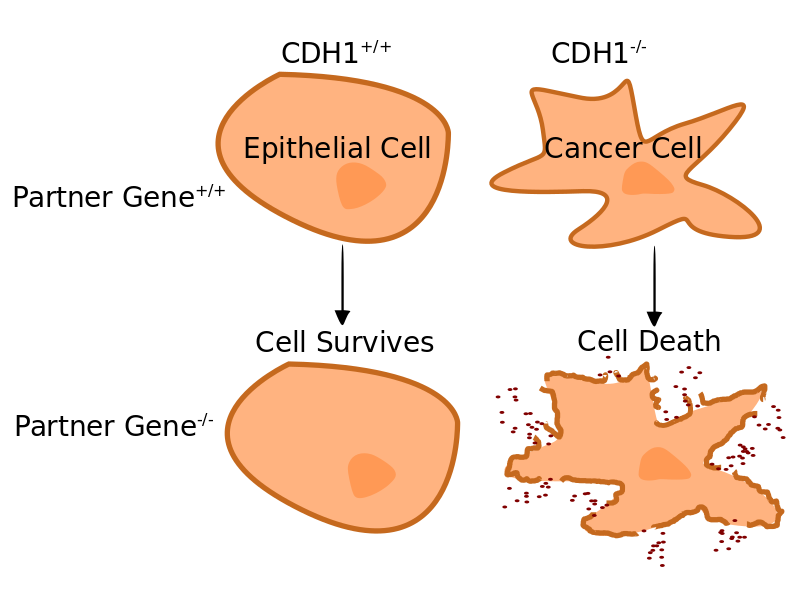
\includegraphics{SL_Concept_no_border.png}
   }
      \caption[Synthetic lethality in cancer]{\textbf{Synthetic lethality in cancer.} Rationale of exploiting synthetic lethality for specifity against a tumour suppressor gene (e.g.,  \textit{CDH1}) while other cells are spared under the inhibition of an SL partner gene.}
\label{fig:SL_Concept}
\end{figure}

\subsection{Clinical Impact of Synthetic Lethality in Cancer}

%Targeted therapeutics combined with the adoption of genomics to identify mutations have begun to impact upon the clinical treatment of cancers. Early examples of targeted therapies are strikingly effective, such as vemurafenib which has shown promise against \textit{BRAF}(V600E) mutations in melanomas in clinical trials \citep{Ravnan2012} and may be widely applicable despite issues with genetic background and drug resistance \citep{Sun2014,Prahallad2012}. Meanwhile, synthetic lethal drug design to indirectly target inactivated genes in cancer has the potential to drastically accelerate the development of precision cancer medicine \citep{Kaelin2009}.

%Synthetic lethal interaction between \textit{\textit{PARP1}} and the tumour suppressor genes \textit{\textit{BRCA1}} and \textit{\textit{BRCA2}} has been demonstrated in cell line and mouse xenograft models, with promising results in both RNAi and drug inhibition experiments \citep{Bryant2005,Farmer2005}. These interactions have been shown to be clinically relevant, with the \textit{\textit{PARP1}}-targeting drug olaparib exhibiting success in clinical trials involving germline and sporadic \textit{\textit{BRCA1}} or \textit{\textit{BRCA2}} mutations in both breast and ovarian cancers, and resulting in fewer adverse effects than cytotoxic chemotherapy \citep{Tutt2010,Audeh2010}. \textit{\textit{PARP1}} inhibitors have shown anti-cancer activity against mutations in other DNA repair genes such as \textit{PTEN} and have been proposed for chemopreventative applications as an alternative to prophylactic surgery for high risk individuals with germline \textit{BRCA1} or \textit{BRCA2} mutations \citep{Strom2012}. Complications were observed in clinical trials, such as acquired drug resistance, complex modifier interactions with \textit{\textit{PARP1}} inhibitors, and their application integrated with genetic tests across cancers in multiple tissues (most commonly breast and ovarian) \citep{Lord2014}. 

The synthetic lethal interaction of \textit{BRCA1} or \textit{BRCA2} with \textit{PARP1} in breast cancer is an example of how gene interactions are important in cancer, including translation to the clinic. These genetic interactions ienable specific targeting of mutations in \textit{BRCA1} or \textit{BRCA2} tumour suppressor genes with PARP inhibitors by inducing synthetic lethality in breast cancer \citep{Farmer2005}. PARP inhibitors are one of the first targeted therapeutics against a tumour suppressor mutation with success in clinical trials. 

\textit{BRCA1} or \textit{BRCA2} and \textit{PARP1} genes demonstrate the application of the synthetic lethal approach to cancer therapy (Ashworth 2008; Kaelin 2005). \textit{BRCA1} and \textit{BRCA1} are homologous DNA repair genes which have been popularised for their role as tumour suppressors; mutation carriers have high risk of breast and ovarian cancers. The \textit{BRCA1} or \textit{BRCA2} genes, which usually repair DNA or destroy the cell if it cannot be repaired, have inactivating somatic mutations in some familial and sporadic cancers. Poly-ADP-ribose polymerase (PARP) genes are tumour suppressor genes involved in base excision DNA repair. Loss of PARP activity results in single-stranded DNA breaks. However, \textit{PARP1}\textsuperscript{-/-} knockout mice are viable and healthy indicating low toxicity from PARP inhibition \citep{Bryant2005}.  

\citet{Bryant2005} showed that \textit{BRCA2}\textsuperscript{{}-/-} cells were sensitive to PARP inhibition by siRNA of \textit{PARP1} or drug inhibition (which targets \textit{PARP1} and \textit{PARP2}) using Chinese hamster ovary cells, MCF7 and MDA-MB-231 breast cell lines. This effect was sufficient to kill mouse tumour xenografts and showed high specificity to \textit{BRCA2} deficient cells in culture and xenografts. \citet{Farmer2005} replicated these results in embryonic stem cells and showed that \textit{BRCA1}\textsuperscript{{}-/-} cells were also sensitive to PARP inhibition relative to the wild-type with siRNA and drug experiments in cell culture and drug activity against \textit{BRCA1} or \textit{BRCA2} deficient embryonic stem cell mouse xenografts. They found evidence that PARP inhibition causes DNA lesions, usually repaired in wild-type cells, which lead to chromosomal instability, cell cycle arrest, and induction of apoptosis in \textit{BRCA1} or \textit{BRCA2} deficient cells. Therefore, the pathways cooperate to repair DNA giving a plausible mechanism for combined loss as an effective anti-cancer treatment.  

Thus PARP inhibitors have potential to clinical uses against \textit{BRCA1} or \textit{BRCA2} mutations in hereditary and sporadic cancers (Ashworth 2008; Kaelin 2005). PARP inhibition has been found to be effective in cancer patients carrying \textit{BRCA1} or \textit{BRCA2} mutations and some other ovarian cancers, suggesting synthetic lethality between PARP and other DNA repair pathways (Str\"om \& Helleday 2012). This supports the potential for PARP inhibition as a chemo-preventative alternative to prophylactic surgery for high risk individuals with \textit{BRCA1} or \textit{BRCA2} mutations (Str\"om \& Helleday 2012). Hormone-based therapy has also been suggested as a chemo-preventative in such high risk individuals and aromatase inhibitors have completed phase I clinical trials for this purpose (Bozovic-Spasojevic2012). \citet{Str\"om2012} also postulate increased efficacy of PARP inhibitors in the hypoxic DNA-damaging tumour micro-environment.  

A PARP inhibitor, olaparib, showed fewer adverse effects than cytotoxic chemotherapy and anti-tumour activity in phase I trials against \textit{BRCA1} or \textit{BRCA2} deficient familial breast, ovarian, and prostate cancers \citep{Fong2009} and sporadic ovarian cancer \citep{Fong2010}. AstraZeneca has reported phase II trials showing the treatment is effective in \textit{BRCA1} or \textit{BRCA2} deficient breast \citep{Tutt2010} and ovarian cancers \citep{Audeh2010} with a favourable therapeutic window and similar toxicity between carriers of \textit{BRCA1} or \textit{BRCA2} mutations and sporadic cases. AstraZeneca announced that olaparib has begun phase III trials for breast and ovarian cancers in 2013. Mixed results in phase II trials in ovarian cancer are behind the delays addressed by retrospective analysis of the cohort subgroup with confirmed mutation of \textit{BRCA1} or \textit{BRCA2} genes in the tumour; unsurprisingly, these patients, benefit most from the PARP inhibitor treatment and have increased platinum sensitivity in combination treatment. This demonstrates the clinical impact of a well characterised system of synthetic lethality with known cancer risk genes. Synthetic lethality has the benefit of being effective against inactivation of tumour suppressor genes by any means, broader than targeting a particular oncogenic mutation \citep{Kaelin 2005}. The targeted therapy is effective in both sporadic and hereditary \textit{BRCA1} or \textit{BRCA2} deficient tumours acting against an oncogenic molecular aberration across several tissues.  

\subsection[High{}-throughput Screening for Synthetic Lethality]{High-throughput Screening for Synthetic Lethality}

%Candidate hypothesis driven synthetic lethal studies in cancer have been successful in some cases \citep{Farmer2005,Bryant2005,vanPel2013} but potentially meaningful synthetic lethal interactions can also occur between unexpected pathways and with genes involved in different biological functions \citep{Costanzo2011}. Unbiased screening is therefore an appealing strategy to identify synthetic lethal interactions, including those informative of novel biological functions, drug mode-of-action, or amenable to treatment. Current screening in cancer cell lines uses genetic or pharmacological approaches, with RNAi or compound libraries respectively, to discover synthetic lethal interactions \citep{Fece2015}.

%Genetic screens can facilitate the discovery of specific genes interacting with a particular disease gene, identify biomarkers for treatment response, and inform development of targeted therapies (with a known mode-of-action and anticipated mechanisms of resistance). Synthetic lethal screens using RNAi have been applied to many cancer genes in cell line models including \textit{\textit{VHL}} in renal cancer \citep{Jerby2014}, \textit{\textit{FH}} in renal cancer \citep{Boettcher2014}, \textit{\textit{WEE1}} in colorectal cancer \citep{Aarts2015}, and \textit{CDH1} in breast cancer \citep{Telford2015}. While some candidates identified in these screens are consistent with the literature or were successfully validated, RNAi screens are susceptible to false positives and a large number of interaction candidates have not been tested, validated, or replicated \citep{Lu2015,Jerby2014,Boettcher2014,Azorsa2009}.

%Chemical screens are a complementary approach that can be used to screen for compounds effective against a particular mutation. While these identify lead compounds with specific activity against mutants, such screens do not ensure compounds are bioavailable, have known mode-of-action, or are selective against a particular target gene and key drug classes are not tested \citep{Fece2015,Kaelin2005,Chan2011}. Despite this, synthetic lethal screens have become widely used for functional genomics and translational  research to identify potential targets for drug development \citep{Fece2015,Telford2015,Jerby2014,Boettcher2014,vanderMeer2014}.

%relevance?
%%%%%%%%%%%
%Genomic and pharmacological screens are becoming widely used for biomedical research despite many potential sources of error \citep{Fece2015,Kaelin2009,Chan2011}.  Off-target effects \citep{Kaelin2005,Chan2011,Fece2015} and growth inhibition \citep{Diehl2014}, from delivery of potentially selective agents, is an issue with RNAi experiments screening for differential viability between cell lines or treatment conditions such as synthetic lethal screens. Mechanisms of gene inhibition, particularly transient gene knockdown in RNAi screens, differ considerably from the behaviour inhibitors in the clinic \citep{Kaelin2009}. Screens are biased  towards genes which are amenable to inhibition, particularly chemical screens which are over-represented for gene functions with existing drugs inhibitors \citep{Chan2011}. Mutations, RNA knockdown, and drug inhibition have different effects on gene function, so perhaps unsurprisingly, synthetic lethal interactions often fail to replicate across experimental systems, cell lines, tissue types, or species \citep{Kaelin2009,Dixon2009}. Several alternatives have been raised to overcome some of these shortcomings of synthetic lethal screens including genome-wide screens with episomal gene transfer \citep{Chan2011}, lentiviral RNAi \citep{Diehl2014}, or CRISPR/\textit{Cas9} genome editing \citep{Fece2015,Shalem2015,Hart2015,Thompson2015}. However, these do not preclude the possibility of off-target effects or account for diverse genetic backgrounds or tumour heterogeneity \citep{Fece2015}.
%%%%%%%%%%%%
%% to consider (here or discussion): off-targets (even with newer tech), differences in KO mechanism -> effect, lack of reproducibility/validations of candidates


The function of signalling pathways and combinations of interacting genes are important in cancer research but classical genetics approaches have been limited to non-redundant pathways \citep{Fraser2004}. The emerging RNAi technologies have vastly expanded the potential for studying genetic redundancy in mammalian experimental models including testing experimentally for synthetic lethality \citep{Fraser2004}. Identifying synthetic lethality is crucial to study gene function, drug mechanisms, and design novel therapies \citep{Lum2004}. Candidate selection of synthetic lethal gene pairs relevant to cancer has shown some success but is limited because interactions are difficult to predict; they can occur between seemingly unrelated pathways in model organisms \citep{Costanzo2011}. While biologically informed hypotheses have had some success in synthetic lethal discovery \citep{Bitler2015, Bryant2005, Farmer2005}, interactions occurring indirectly between distinct pathways would be missed \citep{Boone2007, Costanzo2011}. Scanning the entire genome for interactions against a clinically relevant gene is an emerging strategy being explored with high-throughput screens \citep{Fece2015} and computational approaches \citep{Boucher2013, vanSteen2011}.  

Experimental screening for synthetic lethality is an appealing strategy for wider discovery of functional interactions \textit{in vivo} despite many potential sources of error which must be considered. The synthetic lethal concept has both genetic and pharmacological screening applications to cancer research. Genetic screens, with RNAi to discover the specific genes involved, inform development of targeted therapies with a known mode of action, anticipated mechanisms of resistance, and biomarkers for treatment response. RNAi is a transient knockdown of gene expression more similar to the effect of drugs than complete gene loss and makes comparison to screens in model organisms difficult \citep{Bussey2006}. The RNAi gene knockdown process has inherent toxicity to some cells, potential off-target effects, and issues with a high false positive rate. Therefore, it is important to validate any candidates in a secondary screen and replicate knockdown experiments with a number of independent shRNAs. Alternative gene knockout procedures have also been proposed for synthetic lethal screening including a genome-wide application of the CRIPR/Cas9/sgRNA genome editing technology \citep{Sander2014}, episomal gene transfer \citep{Vargas2004}, or RNAi with lentiviral transfection for delivery of shRNA \citep{Telford2015}. Genetic screens have potential for quantitative gene disruption experiments to selectively target overexpressed genes in cancer via synthetic dosage lethality. While powerful for understanding fundamental cellular function, analysis of isogenic cell lines is inherently limited by assuming only a single mutation differs between them despite susceptibility to ``genetic drift'' and cannot account for diverse genetic backgrounds or tumour heterogeneity \citep{Fece2015}. Genetic screens thus identify targets to develop or repurpose targeted therapies for disease but alone will not directly identify a lead compound to develop for the market or clinical translation.  

Chemical screens are immediately applicable to the clinic by directly screening for selective lead compounds with suitable pharmacological properties. However chemical screens lack a known mode of action, may affect many targets, and screen a narrow range of genes with existing drugs. With either approach there are many challenges translating candidates into the clinic such as finding targets relevant to a range of patients, validation of targets, accounting for a range of genetic (and epigenetic) contexts or tumour micro-environment, identifying effective synergistic combinations, enhancers of existing radiation or cytotoxic treatments, avoiding inherent or acquired drug resistance, and developing biomarkers for patients which will respond to synthetic lethal treatment, including integrating these into clinical trials and clinical practice. Identifying specific target genes is an effective way to anticipate such challenges, which can be approached with genetic screens, so we will focus on these and computational alternatives. Screening methods have proven a fruitful area of research, despite being costly, laborious, and having many different sources of error. These limitations suggest a need for complementary computational approaches to synthetic lethal discovery.  

\subsubsection[Examples of High{}-throughput Synthetic Lethal Screens]{Examples of High-throughput Synthetic Lethal Screens}

Overexpression of genes is another suitable application for synthetic lethality since overexpressed genes cannot be distinguished from the wild-type by direct sequence specific targeted therapy. Overexpression of oncogenes, such as \textit{EGFR}, \textit{MYC}, and \textit{PIM1}, has been found to drive many cancers. \textit{PIM1} is a candidate for synthetic lethal drug design in lymphomas and prostate cancers, where it interacts with \textit{MYC} to drive cancer growth. \citet{vanderMeer2014} performed an RNAi screen to for synthetic lethality between \textit{PIM1} overexpression and gene knockdown in RWPE prostate cancer cell lines. They recognise RNAi screens are valuable for finding therapeutic targets and biomarkers for therapeutic response. \textit{PLK1} gene knockdown and drug inhibition was an effective as a specific inhibitor of \textit{PIM1} overexpressing prostate cells in cell culture and mouse tumour xenografts. \textit{PLK1} inhibition reduced \textit{MYC} expression in pre-clinical models, consistent with expression in human tumours which \textit{PIM1} and \textit{PLK1} are co-expressed and correlated with tumour grade. Therefore \textit{PLK1} is justified as a candidate for drug target against prostate cancer progression.  

Hereditary leiomyomatosis and renal cell carcinoma (HLRCC) is a cancer syndrome of predisposition to benign tumours in the uterus and risk of malignant cancer of the kidney attributed to inherited mutations in fumarate hydratase (\textit{FH}). \citet{Boettcher2014} performed an RNAi screen on HEK293T renal cells for synthetic lethality with \textit{FH}. They found enrichment of haem metabolism (consistent with the literature) and adenylate cyclase pathways (consistent with cAMP dysregulation in \textit{FH} mutant cells). Synthetic lethality between \textit{FH} mutation and adenylate cyclases was validated with gene knockdown, drug experiments, and replicated across both HEK293T renal cells and VOK262 cells derived from a HLRCC patient, suggesting new potential treatments against the disease. Therefore, synthetic lethality is applicable to metabolic dysregulation in cancer, consistent with the Warburg hypothesis (Warburg 1956), and successfully identifies specific anti-cancer drugs, even when the mechanism is unclear. 

Similarly, hereditary diffuse gastric cancer (HDGC) is a cancer syndrome of predisposition to early-onset malignant stomach and breast cancers attributed to mutations in E-Cadherin (\textit{CDH1}). \citet{Telford2015} performed an RNAi screen on MCF10A breast cells for synthetic lethality with \textit{CDH1}. They found enrichment of G-protein coupled receptors (GPCRs) and cytoskeletal gene functions. The results were consistent with a concurrent drug compound screen with a number of candidates validated by lentiviral shRNA gene knockdown and drug testing including inhibitors of Janus kinase, histone deacetylases, phosphoinositide 3-kinase, aurora kinase, and tyrosine kinases. Therefore the synthetic lethal strategy has potential for clinical impact against HDGC, with particular interest in interventions with low adverse effects for chemo-prevention, including repurposing existing approved drugs for activity against \textit{CDH1} deficient cancers.  

RNAi screening for synthetic lethality is also useful for functional genetics to understand drug sensitivity. \citet{Aarts2015} screened WiDr colorectal cells for synthetic lethality between \textit{WEE1} inhibitor treatment and an RNAi library of 1206 genes with functions known to be amenable to drug treatment or important in cancer such as kinases, phosphatases, tumour suppressors, and DNA repair (a pathway \textit{WEE1} regulates). Screening identified a number of synthetic lethal candidates including genes involved in cell cycle regulation, DNA replication, repair, homologous recombination, and Fanconi anaemia. Synthetic lethality with cell-cycle and DNA repair genes was consistent with the literature and validation in a panel of breast and colorectal cell lines supported checkpoint kinases, Fanconi anaemia, and homologous recombination as synthetic lethal partners of \textit{WEE1}. These results show that synthetic lethality can be used to improve drug sensitivity as a combination treatment, especially to exploit genomic instability and DNA repair, which are known to be clinically applicable from previous results with \textit{BRCA1} or \textit{BRCA2} genes and PARP inhibitors \citep{Lord2014}. Therefore, \textit{WEE1} inhibitors are an example of treatment which could be repurposed with the synthetic lethal strategy and similar findings would be valuable to clinicians as a source of biomarkers and novel treatments. While using a panel of cell lines to replicate findings across genetic background is a promising approach to ensure wide clinical application of validated synthetic lethal partners, a computational approach may be more effective as it could account for wider patient variation than scaling up intensive experiments on a wide array of cell lines and could screen beyond limited candidates from an RNAi library.  

Chemical genetic screens are also a viable strategy to identify therapeutically relevant synthetic lethal interactions. \citet{Bitler2015} investigated \textit{ARID1A} mutations, aberrations in chromatin remodelling known to be common in ovarian cancers, for drug response. Ovarian RMG1 cells were screened for drug response specific to \textit{ARID1A} knockdown cells. They used \textit{ARID1A} gene knockdown for consistent genetic background, with control experiments and 3D cell culture to ensure relevance to drug activity in the tumour micro-environment. Screening a panel of commercially available drugs targeting epigenetic regulators found \textit{ESH2} methyltransferase inhibitors effective and specific against \textit{ARID1A} mutation with validation in a panel of ovarian cell lines. Synthetic lethality between \textit{ARID1A} and \textit{ESH2} was supported by decreases in H3K27Me3 epigenetic marks and markers of apoptosis in response to \textit{ESH2} inhibitors. This was mechanistically supported with differential expression of \textit{PIK3IP1} and association of both synthetic lethal genes with the \textit{PIK3IP1} promoter identifying the P1I3K-AKT signalling pathway as disrupted when both genes are inhibited. This successfully demonstrates the importance of synthetic lethality in epigenetic regulators, identifies a therapeutically relevant synthetic lethal interaction, and shows that chemical genetic screens could model drug response and combination therapy in cancer cells. However this approach is limited to finding synthetic lethal interactions between genes with known similar function, which may not be the most suitable for treatment. Further limiting experiments to genes with existing targeted drugs reduces the number of synthetic lethal interactions detected, assumes on their drug specificity to a particular target, and many of these drugs are not clinically available yet anyway as they are still in clinical trials for other diseases or are not supported by healthcare systems in many countries.  

\citet{Jerby2014} combined a computational approach to triage candidates with a conventional RNAi screen to validate synthetic lethal partners. They screened a selection of computationally predicted candidates and randomly selected genes with RNAi against \textit{VHL} loss of function mutation in RCC4 renal cell lines. The computational method had a high AUROC of 0.779 and predictions were enriched 4x for validated RNAi hits over randomly selected genes. This approach detected known synthetic lethal pairs such as \textit{BRCA1} or \textit{BRCA2} genes with \textit{PARP1} and \textit{MSH2} with \textit{DHFR}. The synthetic lethal candidates identified with both RNAi screening and computational prediction formed an extensive network of 2077 genes with 2816 synthetic lethal interactions and similar network of 3158 genes with 3635 synthetic dosage lethal interactions (for synthetic lethality with over-expression). Each network was scale-free as expected of a biological network and was enriched for known cancer genes, essential genes in mice, and could be harnessed for predicting prognosis and drug response. While demonstrating the feasibility of combining experimental and computational approaches to synthetic lethality in cancer, there remain challenges in predicting synthetic lethal genes, novel drug targets, and translation into the clinic.  

The examples above show that high-throughput screens are an effective approach to discover synthetic lethality in cancer with a wide range of applications. Screens are more comprehensive than hypothesis-driven candidate gene approaches and successfully find known and novel synthetic lethal interactions with potential for rapid clinical application. They have the power to test mode of action of drugs, find unexpected synthetic lethal interactions between pathways, or identify effective treatment strategies without needing a clear mechanism. However, synthetic lethal screens are costly, labour-intensive, error-prone, and biased towards genes with effective RNAi knockdown libraries. Limited genetic background, lethality to wild-type cell during gene knockdown, off-target effects, and difficultly replicating synthetic lethality across different cell lines, tissues, laboratories, or conditions stems from a high false positive rate and a lack of standardised thresholds to identify synthetic lethality in a high-throughput screen. Therefore there is a need for replication, validation, and alternative approaches to identify synthetic lethal candidates. Varied conditions between experimental screens and differences between RNAi or drug screens makes meta-analysis difficult. Thus genome-scale synthetic lethal experiments are not feasible, even in model organisms, so a computational approach would be more suitable for this task.  

\subsection[Computational Prediction of Synthetic Lethality]{Computational Prediction of Synthetic Lethality}

%Computational approaches to identifying synthetic lethal interactions are rapidly developing into a feasible addition to genomic screens due to the low cost, reliable automated reproducible workflows, ability to account for distinct genetic backgrounds, and lack of off-target effects or bias towards particular genes \citep{Boucher2013, Thompson2015}. 
%%%%%%%%relevance
%Synthetic lethal prediction has been widely explored in model organisms - a key example is the task of inferring the entire gene network from incomplete synthetic lethal networks and functional genomics data in \textit{Saccharomyces cerevisiae} \citep{Boucher2013}. However, synthetic lethal interactions are difficult to reproduce across species \citep{Dixon2009,Lehner2006}, not all of the data types used for prediction of synthetic lethal interactions in available in humans, and the methods assuming conserved network structure may not be applicable to unstable cancer systems. Computational approaches to discovery of synthetic lethal interactions tailored to mammals, or specifically to human cancers, are therefore needed for applicable results. However, many existing computational approaches are difficult to apply to novel genes having been trained on known gene functions, using complex machine learning methods, or are over-represented for genes where single gene aberrations have large effects on cellular phenotypes such as \textit{\textit{TP53}} or \textit{AKT}.
%%%%%%% join to next paragraph
%Analysis of gene expression is an appealing strategy for discovery of synthetic lethal interactions in cancer due to the widespread availability of data for different cancers, lack of bias towards well characterised genes, and potential further use for expression of interacting partners as biomarkers for treatment with drugs designed to exploit them.

%A recent example of a computational tool for identification of synthetic lethal interactions using gene expression analysis is the DAISY methodology \citep{Ryan2014,Crunkhorn2014}, which combines predictions from patient samples  of The Cancer Genome Atlas (TCGA), cell lines of the Cancer Cell Line Encyclopaedia (CCLE), and RNAi validation experiments \citep{Jerby2014}. The predictors of synthetic lethality were genomic `survival of the fittest' (using DNA copy number and somatic mutation in patient and cell lines data), `functional examination' of gene essentiality (using RNA interference data in cell cell lines), and pairwise `gene co-expression' (in cell lines).

%%%%%%%% edit to tone down anti-DAISY message  restructure paragraphs to fewer ideas apiece
%As a proof-of-concept, DAISY demonstrates the potential of bioinformatics approaches to generate synthetic lethal candidates against the tumour suppressor \textit{\textit{VHL}} in a renal cancer cell line, along with reasonable statistical performance and generalisation to gene essentiality, genetic dosage, or drug analyses \citep{Jerby2014}. However, DAISY partners of \textit{\textit{VHL}} showed only modest 4-fold over-represent\-ation in validated shRNA screening than a screen of random genes and the method has not been widely adopted in studies of other cancer genes.
%%criticism of DAISY moved to discussion

%An alternative to the approach is the use of `cancer genome evolution' to predict synthetic lethal genes from their behaviour in genomics data\citep{Lu2015}, as the induced essentiality of remaining synthetic lethal partners takes effect in the tumour progression. Lu \textit{et al.} \citep{Lu2015} postulate that, in response to loss of a gene function, a tumour would would either resist by maintaining low expression or compensate by increasing the activity of synthetic lethal partner genes. This model predicted far more genes than previous attempts at discovery of synthetic lethal interactions, performed well at a genome-wide scale, and produced a higher 14-fold over-represent\-ation of validated synthetic lethal pairs. While Lu \textit{et al.} \citep{Lu2015} provide a comprehensive list of their strongest candidate synthetic lethal pairs across cancer types, these do not include \textit{CDH1}, thus there remains a need for computational predictions for this gene and a tool other researchers may use for similar screen triage purposes against a candidate gene in a specific cancer.  


%% (Re)move the below paragraph? Too negative / irrelevant?
%These prior approaches used complex cutting-edge machine learning techniques which may be difficult for the biological community to adopt and DNA copy number which may not be available for many  applications \citep{Jerby2014, Lu2015}. %% may be speculation
%Here, we present a synthetic lethal analysis based solely on gene expression data which could feasibly be applied to studies of other genes to utilise the large number of samples collected for many genes in diseases such as cancers.  We use the example of \textit{CDH1} as a tumour suppressor gene in breast cancer samples from TCGA \citep{TCGA2012} to highlight the importance of synthetic lethal interactions, potential relationships between them, and the biological pathways involved.
%R code for our synthetic lethal analysis will be avaialable on our \href{https://github.com/TomKellyGenetics/slipt}{GitHub repository} as an R package. 


Prediction of gene interaction networks is a feasible alternative to high-throughput screening with biological importance and clinical relevance. There are many existing methods to predict gene networks, as reviewed by \citet{vanSteen2011} and \citet{Boucher2013}, summarised in Table \ref{tab:methods_model} below. However, many of these methods have limitations including the requirement for existing SGI data, several data inputs, and reliability of gene function annotation. Many of the existing methods also assume conservation of individual interactions between species, which has been found not to hold in yeast studies \citep{Dixon2008}. Tissue specificity is important in gene regulation and gene expression, which are used as predictors of genetic interaction. However, tissue specificity of genetic interactions cannot be explored in yeast studies and has not been considered in any of the following studies of multicellular model organisms, human networks, or cancers. Similarly, investigation into tissue specificity of protein-protein interactions (PPIs) , an important predictor of genetic interactions, is difficult given the high-throughput two-hybrid screens occur out of cellular context for multicellular organisms.  

\begin{table*}[!ht]
\caption{Existing prediction methods for Genetic Interaction Networks in Model Organisms}
\label{tab:methods_model}
%\begin{center}
\resizebox{ \textwidth}{!}{
\begin{supertabular}{l|l|l|l|l}

\multicolumn{1}{m{4.421cm}}{\cellcolor{white}\bfseries\color{black}
Method} &
\multicolumn{1}{m{2.342cm}}{\cellcolor{white}\color{black}
\textcolor{black}{Input Data}} &
\multicolumn{1}{m{2.388cm}}{\cellcolor{white}\color{black}
\textcolor{black}{Species}} &
\multicolumn{1}{m{4.552cm}}{\cellcolor{white}\bfseries\color{black}
Source} &
\cellcolor{white}\bfseries\color{black} Tool Offered\\\hline
\cellcolor[rgb]{0.8509804,0.8862745,0.9529412}\color{black}
\textcolor{black}{Between Pathways Model} &
\cellcolor[rgb]{0.8509804,0.8862745,0.9529412}\color{black} PPI, SGI &
\cellcolor[rgb]{0.8509804,0.8862745,0.9529412}\color{black}
\textit{\textcolor{black}{S. cerevisiae}} &
\cellcolor[rgb]{0.8509804,0.8862745,0.9529412}\color{black}
\citet{Kelley2005} &
\cellcolor[rgb]{0.8509804,0.8862745,0.9529412}~
\\\hline
Within Pathways Model &
PPI, SGI &
\textit{S. cerevisiae} &
\citet{Kelley2005} &
~
\\\hline
\cellcolor[rgb]{0.8509804,0.8862745,0.9529412}\color{black}
\textcolor{black}{Decision Tree} &
\cellcolor[rgb]{0.8509804,0.8862745,0.9529412}\color{black} PPI,
expression, phenotype &
\cellcolor[rgb]{0.8509804,0.8862745,0.9529412}\color{black}
\textit{\textcolor{black}{S. cerevisiae}} &
\cellcolor[rgb]{0.8509804,0.8862745,0.9529412}\color{black}
\citet{Wong2004} &
\cellcolor[rgb]{0.8509804,0.8862745,0.9529412}\color{black} 2
Hop\\\hline
Logistic Regression &
SGI, PPI, co-expression, phenotype &
\textit{C. elegans} &
\cite{Zhong2006} &
Gene Orienteer\\\hline
\cellcolor[rgb]{0.8509804,0.8862745,0.9529412}\color{black}
\textcolor{black}{Network Sampling} &
\cellcolor[rgb]{0.8509804,0.8862745,0.9529412}\color{black} SGI, PPI, GO
&
\cellcolor[rgb]{0.8509804,0.8862745,0.9529412}\color{black}
\textit{\textcolor{black}{S. cerevisiae}} &
\cellcolor[rgb]{0.8509804,0.8862745,0.9529412}{
\begin{tabular}{l@{}l@{}}\color{black}\citet{LeMeur2008} \\ \color{black}\citet{LeMeur2014}\end{tabular}}
&
\cellcolor[rgb]{0.8509804,0.8862745,0.9529412}\color{black}
SLGI(R)\\\hline
Random Walk &
GO, PPI, expression &

\begin{tabular}{l@{}l@{}}\textit{S. cerevisiae} \\ \textit{C. elegans}\end{tabular}
 &
\citet{Chipman2009} &
~
\\\hline
\cellcolor[rgb]{0.8509804,0.8862745,0.9529412}\color{black}
\textcolor{black}{Shared Function} &
\cellcolor[rgb]{0.8509804,0.8862745,0.9529412}\color{black}
Co-expression, PPI, text mining, phylogeny &
\cellcolor[rgb]{0.8509804,0.8862745,0.9529412}\color{black}
\textit{\textcolor{black}{C. elegans}} &
\cellcolor[rgb]{0.8509804,0.8862745,0.9529412}\color{black}
\citet{Lee2010b} &
\cellcolor[rgb]{0.8509804,0.8862745,0.9529412}\color{black}
WormNet\\\hline
Logistic Regression &
Co-expression, PPI, phenotype &
\textit{C. elegans} &
\citet{Lee2010a} &
GI Finder\\\hline
\cellcolor[rgb]{0.8509804,0.8862745,0.9529412}\color{black}
\textcolor{black}{Jaccard Index} &
\cellcolor[rgb]{0.8509804,0.8862745,0.9529412}\color{black} GO, SGI,
PPI, phenotype &
\cellcolor[rgb]{0.8509804,0.8862745,0.9529412}\color{black} Eukarya &
\cellcolor[rgb]{0.8509804,0.8862745,0.9529412}\color{black}
\citet{Hoehndorf2013} &
\cellcolor[rgb]{0.8509804,0.8862745,0.9529412}~
\\\hline
Bimodal Statistics &
~
 &
~
 &
\cite{Wappett2014} &
BiSEp(R)\\\hline
\cellcolor[rgb]{0.8509804,0.8862745,0.9529412}\color{black}
\textcolor{black}{Machine Learning} &
\cellcolor[rgb]{0.8509804,0.8862745,0.9529412}~
 &
\cellcolor[rgb]{0.8509804,0.8862745,0.9529412}~
 &
\cellcolor[rgb]{0.8509804,0.8862745,0.9529412}
\begin{tabular}{l@{}l@{}}\color{black} Discussed by \citep{Babyak2004} \\and \citet{Lee2009} \end{tabular}

 &
\cellcolor[rgb]{0.8509804,0.8862745,0.9529412}~
\\\hline
\begin{tabular}{l@{}l@{}}\color{black} Machine Learning \\as discussed by \citet{Wu2014}  \end{tabular}
&
~
 &
~
 &

\begin{tabular}{l@{}l@{}l@{}}
\citet{Qi2008} \\
\citet{Paladugu2008} \\
\citet{Li2011}
\end{tabular}
&
~
\\\hline
\cellcolor[rgb]{0.8509804,0.8862745,0.9529412}\color{black}
\textcolor{black}{Machine Learning} &
\cellcolor[rgb]{0.8509804,0.8862745,0.9529412}~
 &
\cellcolor[rgb]{0.8509804,0.8862745,0.9529412}~
 &
\cellcolor[rgb]{0.8509804,0.8862745,0.9529412}\color{black}
\citet{Pandey2010} &
\cellcolor[rgb]{0.8509804,0.8862745,0.9529412}\color{black} MNMC\\\hline
Machine Learning Meta-Analysis &
~
 &
~
 &
\cite{Wu2014} &
MetaSL\\\hline
\cellcolor[rgb]{0.8509804,0.8862745,0.9529412}{\color{black}
\begin{tabular}{l@{}l@{}l@{}}
\textcolor{black}{Flux Variability Analysis} \\
\textcolor{black}{Flux Balance Analysis} \\
\textcolor{black}{Network Simulation}
\end{tabular}
} &
\cellcolor[rgb]{0.8509804,0.8862745,0.9529412}\color{black} Metabolism &
\cellcolor[rgb]{0.8509804,0.8862745,0.9529412}{\color{black}

\begin{tabular}{l@{}l@{}}
\textit{\textcolor{black}{E. coli}} \\
\color{black} \textit{\textcolor{black}{Mycoplasma pneumoniae}}
\end{tabular}
} &
\cellcolor[rgb]{0.8509804,0.8862745,0.9529412}\color{black}
\citet{G\"uell2014} &
\cellcolor[rgb]{0.8509804,0.8862745,0.9529412}~
\\\hline
\end{supertabular}
}
%\end{center}
\end{table*}

%\begin{flushleft}
%\resizebox{\textwidth}{!}{
%\begin{tabular}{m|m|m|m|m}

%\begin{table*}[!ht]
%\caption{Existing prediction methods for Synthetic Lethality}
%\label{tab:methods_SL}
%\begin{center}
%\resizebox{ \textwidth}{!}{
%\begin{supertabular}{l|l|l|l|l}

\begin{table*}[!ht]
\caption{Existing prediction methods for Synthetic Lethality}
\label{tab:methods_SL}
%\begin{center}
\resizebox{ \textwidth}{!}{
\begin{tabular}{l|l|l|l|l}
\multicolumn{1}{m{4.421cm}}{\cellcolor{white}\bfseries\color{black}
Method} &
\multicolumn{1}{m{2.342cm}}{\cellcolor{white}\color{black}
\textcolor{black}{Input Data}} &
\multicolumn{1}{m{2.388cm}}{\cellcolor{white}\color{black}
\textcolor{black}{Species}} &
\multicolumn{1}{m{4.552cm}}{\cellcolor{white}\bfseries\color{black}
Source} &
\cellcolor{white}\bfseries\color{black} Tool Offered\\\hline
\cellcolor[rgb]{0.8509804,0.8862745,0.9529412}\color{black}
\textcolor{black}{Network Centrality} &
\cellcolor[rgb]{0.8509804,0.8862745,0.9529412}\color{black} PPI &
\cellcolor[rgb]{0.8509804,0.8862745,0.9529412}\color{black}
\textit{\textcolor{black}{H. sapiens}} &
\cellcolor[rgb]{0.8509804,0.8862745,0.9529412}\color{black}
\citet{Kranthi2013} &
\cellcolor[rgb]{0.8509804,0.8862745,0.9529412}~
\\\hline
Differential Expression &
\begin{tabular}{l@{}l@{}}
Expression \\
Mutation
\end{tabular}
&
\textit{H. sapiens} &
\citet{Wang2013} &
~
\\\hline
\cellcolor[rgb]{0.8509804,0.8862745,0.9529412}{\color{black}

\begin{tabular}{l@{}l@{}}
\textcolor{black}{Comparative Genomics} \\
\color{black} \textcolor{black}{Chemical-Genomics}
\end{tabular}
}
 &
\cellcolor[rgb]{0.8509804,0.8862745,0.9529412}

\begin{tabular}{l@{}l@{}}
Yeast SGI \\
Homology
\end{tabular}
 &
\cellcolor[rgb]{0.8509804,0.8862745,0.9529412}\color{black}
\textit{\textcolor{black}{H. sapiens}} &
\cellcolor[rgb]{0.8509804,0.8862745,0.9529412}\color{black}
\citet{Heiskanen2012} &
\cellcolor[rgb]{0.8509804,0.8862745,0.9529412}~
\\\hline
Comparative Genomics &
\begin{tabular}{l@{}l@{}}
Yeast SGI \\
Homology
\end{tabular}
 &
\textit{H. sapiens} &
\citet{Deshpande2013} &
~
\\\hline
\cellcolor[rgb]{0.8509804,0.8862745,0.9529412}\color{black}
\textcolor{black}{Genome Evolution} &
\cellcolor[rgb]{0.8509804,0.8862745,0.9529412}~
 &
\cellcolor[rgb]{0.8509804,0.8862745,0.9529412}~
 &
\cellcolor[rgb]{0.8509804,0.8862745,0.9529412}\color{black}
\citet{Lu2013} &
\cellcolor[rgb]{0.8509804,0.8862745,0.9529412}~
\\\hline
Machine Learning &
~
 &
~
 &
\begin{tabular}{l@{}l@{}}\color{black} Discussed by \citet{Babyak2004} \\and \citet{Lee2009} \end{tabular}

 &
~
\\\hline
\cellcolor[rgb]{0.8509804,0.8862745,0.9529412}\color{black}
\textcolor{black}{Differential Expression} &
\cellcolor[rgb]{0.8509804,0.8862745,0.9529412}~
 &
\cellcolor[rgb]{0.8509804,0.8862745,0.9529412}~
 &
\cellcolor[rgb]{0.8509804,0.8862745,0.9529412}\color{black}
\citet{Tiong2014} &
\cellcolor[rgb]{0.8509804,0.8862745,0.9529412}~
\\\hline
Literature Database &
~
 &
~
 &
\citet{Li2014)} &
Syn-Lethality\\\hline
\cellcolor[rgb]{0.8509804,0.8862745,0.9529412}\color{black}
\textcolor{black}{Meta-Analysis} &
\cellcolor[rgb]{0.8509804,0.8862745,0.9529412}\color{black}
\begin{tabular}{l@{}l@{}}
Meta-Analysis \\
Machine Learning
\end{tabular}
 &
\cellcolor[rgb]{0.8509804,0.8862745,0.9529412}~
 &
\cellcolor[rgb]{0.8509804,0.8862745,0.9529412}\color{black}
\citet{Wu2014} &
\cellcolor[rgb]{0.8509804,0.8862745,0.9529412}\color{black}
MetaSL\\\hline
Pathway Analysis &
~
 &
~
 &
\citet{Zhang2015} &
~
\\\hline
\cellcolor[rgb]{0.8509804,0.8862745,0.9529412}\color{black}
\textcolor{black}{Protein Domains} &
\cellcolor[rgb]{0.8509804,0.8862745,0.9529412}\color{black} Homology &
\cellcolor[rgb]{0.8509804,0.8862745,0.9529412}~
 &
\cellcolor[rgb]{0.8509804,0.8862745,0.9529412}\color{black}
\citet{Kozlov2015} &
\cellcolor[rgb]{0.8509804,0.8862745,0.9529412}~
\\\hline
Data-Mining &
~
 &
~
 &
\begin{tabular}{l@{}l@{}l@{}l@{}}
\citet{Jerby-Arnon2014}\\
\citet{Ryan2014} \\
\citet{Crunkhorn2014} \\
\citet{Lokody2014}\end{tabular}

&
DAISY (method)\\\hline
\cellcolor[rgb]{0.8509804,0.8862745,0.9529412}{\color{black}

\begin{tabular}{l@{}l@{}l@{}}
\textcolor{black}{Cancer Genome Evolution} \\
{\color{black} \textcolor{black}{Hypothesis Test}} \\
\color{black} \textcolor{black}{Machine Learning}
\end{tabular}
} &
\cellcolor[rgb]{0.8509804,0.8862745,0.9529412}{
\begin{tabular}{l@{}l@{}l@{}}
Expression \\
DNA CNV \\
Known SL
\end{tabular}
} &
\cellcolor[rgb]{0.8509804,0.8862745,0.9529412}\color{black}
\textit{\textcolor{black}{H. sapiens}} &
\cellcolor[rgb]{0.8509804,0.8862745,0.9529412}\color{black}
\citet{Lu2015} &
\cellcolor[rgb]{0.8509804,0.8862745,0.9529412}~
\\\hline
Chi-Squared Test &
\begin{tabular}{l@{}l@{}l@{}}
Expression \\
DNA CNV \\
Methylation or Mutation
\end{tabular}
 &
\textit{H. sapiens} &
\begin{tabular}{l@{}l@{}l@{}}
Tom Kelly, Parry Guilford, and Mik Black \\
Dissertation (Kelly 2013) \\
Manuscript in Preparation (2015-2017)
\end{tabular}
&
SLIPT\\\hline
\\\hline
\end{tabular}
}
%\end{center}
\end{table*}

There are a number of existing computational methods for predicting synthetic lethal gene pairs. While these demonstrate the power and need for predictions of synthetic lethality in human and cancer contexts, limitations of previous methods \ could be met with a different approach. For instance, computational approaches to synthetic lethal prediction are often difficult to interpret, replicate for new genes, or reliant on data types not available for genes that other cancer researchers work on.  

\citet{Kranthi2013)} took a network approach to discovery of synthetic lethal candidate selection applying the concept to ``centrality'' to a human PPI network involving interacting partners of known cancer genes. The effect of removing pairs of genes on connectivity of the network was used as a surrogate for viability which is supported by observations that the PPI and synthetic lethal networks are orthogonal in \textit{S. cerevisiae} studies (Tong2004). While they showed the power law distribution expected of a scale-free synthetic lethal network with centrality measures, their approach was limited to known cancer genes and is not applicable to genes without PPI data. Other nucleotide sequencing data types are more commonly available for cancer studies at a genomic scale. Of further concern is that the results were enriched for p53 synthetic lethal partners which is relevant to many cancer researchers but makes using this approach for other cancer genes difficult with respect to multiple testing. This enrichment may be due to the known drastic effect of removing p53 itself from the network as a master regulator, cancer driving tumour suppressor gene, and highly connected network ``hub''. The focus on cancer genes is useful for translation into therapeutics but does not account for variable genetic backgrounds or effect of protein removal on the whole cellular network.  

A comparative genomics approach by \citet{Deshpande2013)} used the results of well characterised high-throughput mutation screens in \textit{S. cerevisiae} as candidates for synthetic lethality in humans \citep{Baryshnikova2010a, Boone2007, Costanzo2010, Costanzo2011, Tong2001, Tong2004}. Yeast synthetic lethal partners were compared to human orthologues to find cancer relevant synthetic lethal candidate pairs with direct therapeutic potential. Proposed as a complementary approach to siRNA screens, several synthetic lethal candidates were successfully validated in cell culture; however, this methodology is limited to application on human genes with known yeast orthologues. Synthetic lethal interactions themselves may not be conserved between species \citep{Dixon2009a}, although synthetic lethal interactions between pathways may are more comparable. There have been many gene duplications in the separate evolutionary histories of humans and yeast which may lead to differences in genetic redundancy. Yeast are further not an ideal human cancer model because they are do not have tissue specificity, multicellular gene regulation, or orthologues to a number of known cancer genes such as p53.  

Differential gene expression has also been explored to predict synthetic lethal pairs in cancer which would be widely applicable due to the availability of public gene expression data for a large number of samples and cancer types. \citet{Wang2013} found differentially expressed genes between tumours with or without functional p53 mutations in Cancer Genome Atlas (TCGA) and Cell Line Encyclopaedia (CCLE) RNA-Seq gene expression data as candidate synthetic lethal partner pathways of p53. Some of these pathways were consistent with the literature and drug sensitivity cell-line screens demonstrating the potential of gene expression as a surrogate for gene function and use of public genomic data to predict synthetic lethal gene pairs in cancer. However, the analyses were limited to kinase genes and focused on currently druggable genes, lacking wider application of synthetic lethal prediction methodology. This approach may not be feasible or applicable in cancer genes with a lower mutation rate than p53.  

\citet{Tiong2014)} also investigated gene expression as a predictor of synthetic lethal pairs with colorectal cancer microarrays. Simultaneously differentially expressed ``tumour dependent'' gene pairs between cancer and normal tissue were used as candidate synthetic lethal interactions. The top 20 genes were tested for differential expression at the protein level with immunohistochemistry staining and correlation with clinical characteristics. Some of the predicted synthetic lethal pairs were consistent with the literature and 2 novel synthetic lethal interactions with p53 were validated in pre-clinical models. While a valuable proof-of-concept for integration of \textit{in silico} approaches to synthetic lethal discovery in cancer, the results again focus on p53 rather than the wider application of synthetic lethal prediction. The gene expression analyses were conducted in a Han Chinese population with a small sample size (70 tumour, 12 normal) and may not be applicable to other populations.  

Another approach to systematic synthetic lethality discovery specific to human cancer (in contrast to the plethora of yeast synthetic lethality data) was to build a database as done by \citet{Li2014)}. In their relational database, called ``Syn-lethality'', they have curated both known experimentally discovered synthetic lethal pairs in humans (113 pairs) from the literature and those predicted from synthetic lethality between orthologous genes in \textit{S. cerevisiae} yeast (1114 pairs). This knowledge-based database is the first known dedicated to human cancer synthetic lethal interactions and integrates gene functional, annotation, pathway and molecular mechanism data with experimental and predicted synthetic lethal gene pairs. This combination of data sources is intended to tackle the trade-off between more conclusive synthetic lethal experiments in yeast and more clinically relevant synthetic lethal experiments in human cancer models, such as RNAi, especially when high-throughput screens are costly and prone to false positives in either system and difficult to replicate across gene backgrounds. This database centralises a wealth of knowledge scattered in the literature including cancer relevant genes (\textit{BRCA1}, \textit{BRCA2}, \textit{PARP1}, \textit{PTEN}, \textit{VHL}, \textit{MYC}, \textit{EGFR}, \textit{MSH2}, \textit{KRAS}, and \textit{TP53}) and is publicly available as a Java App. However, the methodology was not released to replicate or add to the findings with new datasets. Suggested future directions were promising, such as constructing networks of known synthetic lethality, applying known synthetic lethality to cancer treatment, data mining, replicating the approach for synthetic lethality in model organisms, signalling pathways, and develop a complete global network in human cancer or yeast (both of which are still incomplete with experimental data).  

From the same group, \citet{Wu2014} developed a meta-analysis method (based on the machine learning methods in Table \ref{tab:tab:methods_meta}) for synthetic lethal gene pairs relevant to developing selective drugs against human cancer. They note that computational approaches scale-up across the genome at lower cost than experimental screens but existing methods are limited by noise and overfitting to a particular predictive feature. Their ``metaSL'' approach performs well with an AUROC of 0.871 with the claimed strengths of existing machine learning methods and the results are shared on the web. However, once again, the method is not available for analysis of other genes studied by the cancer research community and the method lacks mechanisms, reproducibility, and interpretation by researchers. While machine learning has great potential as a predictor, it is difficult to interpret which features are being used for prediction and their mechanistic significance, particularly for biologists with limited exposure to computational concepts.  

Focusing on the potential for synthetic lethality to be an effective anti-cancer drug target, \citet{Zhang2015} used modelling signalling pathways to identify synthetic lethal interactions between known drug targets and cancer genes. A computational approach was again used here to tackle the limitations of experimental RNAi screens such as scale, instability of knockdown, and off-target effects. Strangely, they seemed more concerned with the needs of the pharmaceutical companies than those of the patients. However, their `hybrid' method of a data-driven model and known signalling pathways showed potential as a means to predict cell death in single and combination gene knockouts. They used time series gene expression data \citep{Lee2012} and pathways (the Gene Ontology system). This approach successfully detected many known essential genes in the human gene essentiality database, known synthetic lethal partners in the Syn-Lethality database, and predicted novel synthetic lethal gene pairs. Novel results were enriched for \textit{TP53} and AKT synthetic lethal partners, genes known to be important in many cancers but also predicted to be essential by single gene disruption having a large impact on the signalling pathways. Notably, they claim to be able to detect all 3 types of functionally related pathways or protein complexes. The results are consistent with the experimental results in the literature but the group has not shown validation for novel synthetic lethal interactions.  

\begin{table*}[!ht]
\caption{Existing Computational Methods used for meta-analysis by \citet{Wu2014}
\label{tab:methods_meta}
%\begin{center}
\resizebox{ \textwidth}{!}{
\begin{tabular}{l|l|l|l|l}
\multicolumn{1}{m{4.421cm}}{\cellcolor{white}\bfseries\color{black}
Method} &
\multicolumn{1}{m{2.342cm}}{\cellcolor{white}\color{black}
\textcolor{black}{Input Data}} &
\multicolumn{1}{m{2.388cm}}{\cellcolor{white}\color{black}
\textcolor{black}{Species}} &
\multicolumn{1}{m{4.552cm}}{\cellcolor{white}\bfseries\color{black}
Source} &
\cellcolor{white}\bfseries\color{black} Tool Offered\\\hline
\cellcolor[rgb]{0.8509804,0.8862745,0.9529412}\color{black}
\textcolor{black}{Random Forest} &
\cellcolor[rgb]{0.8509804,0.8862745,0.9529412}\color{black} Machine
Learning &
\cellcolor[rgb]{0.8509804,0.8862745,0.9529412}\color{black}
\textit{\textcolor{black}{H. sapiens}} &
\cellcolor[rgb]{0.8509804,0.8862745,0.9529412}{\color{black}
\citet{Hall2009}}

\color{black} \citet{Breiman2001} &
\cellcolor[rgb]{0.8509804,0.8862745,0.9529412}\color{black} WEKA\\\hline
J48 (decision tree) &
Machine Learning &
\textit{H. sapiens} &
\citet{Hall2009}

~
 &
WEKA\\\hline
\cellcolor[rgb]{0.8509804,0.8862745,0.9529412}\color{black}
\textcolor{black}{Bayes (Log Regression)} &
\cellcolor[rgb]{0.8509804,0.8862745,0.9529412}\color{black} Machine
Learning &
\cellcolor[rgb]{0.8509804,0.8862745,0.9529412}\color{black}
\textit{\textcolor{black}{H. sapiens}} &
\cellcolor[rgb]{0.8509804,0.8862745,0.9529412}{\color{black}
\citet{Hall2009}}

~
 &
\cellcolor[rgb]{0.8509804,0.8862745,0.9529412}\color{black} WEKA\\\hline
Bayes (Network) &
Machine Learning &
\textit{H. sapiens} &
\citet{Hall2009}

~
 &
WEKA\\\hline
\cellcolor[rgb]{0.8509804,0.8862745,0.9529412}\color{black}
\textcolor{black}{PART (Rule-based)} &
\cellcolor[rgb]{0.8509804,0.8862745,0.9529412}\color{black} Machine
Learning &
\cellcolor[rgb]{0.8509804,0.8862745,0.9529412}\color{black}
\textit{\textcolor{black}{H. sapiens}} &
\cellcolor[rgb]{0.8509804,0.8862745,0.9529412}{\color{black}
\citet{Hall2009}}

~
 &
\cellcolor[rgb]{0.8509804,0.8862745,0.9529412}\color{black} WEKA\\\hline
RBF Network &
Machine Learning &
\textit{H. sapiens} &
\citet{Hall2009}

~
 &
WEKA\\\hline
\cellcolor[rgb]{0.8509804,0.8862745,0.9529412}\color{black}
\textcolor{black}{Bagging / Bootstrap} &
\cellcolor[rgb]{0.8509804,0.8862745,0.9529412}\color{black} Machine
Learning &
\cellcolor[rgb]{0.8509804,0.8862745,0.9529412}\color{black}
\textit{\textcolor{black}{H. sapiens}} &
\cellcolor[rgb]{0.8509804,0.8862745,0.9529412}{\color{black}
\citet{Hall2009}}

~
 &
\cellcolor[rgb]{0.8509804,0.8862745,0.9529412}\color{black} WEKA\\\hline
Classification via Regression &
Machine Learning &
\textit{H. sapiens} &
\citet{Hall2009}

~
 &
WEKA\\\hline
\cellcolor[rgb]{0.8509804,0.8862745,0.9529412}\color{black}
\textcolor{black}{Support Vector Machine (Linear)} &
\cellcolor[rgb]{0.8509804,0.8862745,0.9529412}\color{black} Machine
Learning &
\cellcolor[rgb]{0.8509804,0.8862745,0.9529412}\color{black}
\textit{\textcolor{black}{H. sapiens}} &
\cellcolor[rgb]{0.8509804,0.8862745,0.9529412}\color{black}
\citet{Vapnik1995} &
\cellcolor[rgb]{0.8509804,0.8862745,0.9529412}~
\\\hline
Support Vector Machine (RBF -- Gaussian) &
Machine Learning &
\textit{H. sapiens} &
\citet{Joachims1999} &
~
\\\hline
\cellcolor[rgb]{0.8509804,0.8862745,0.9529412}\color{black}
\textcolor{black}{Multi-Network Multi-Class (MNMC)} &
\cellcolor[rgb]{0.8509804,0.8862745,0.9529412}\color{black} Machine
Learning &
\cellcolor[rgb]{0.8509804,0.8862745,0.9529412}\color{black}
\textit{\textcolor{black}{H. sapiens}} &
\cellcolor[rgb]{0.8509804,0.8862745,0.9529412}\color{black}
\citet{Pandey2010} &
\cellcolor[rgb]{0.8509804,0.8862745,0.9529412}~
\\\hline
MetaSL (Meta-Analysis) &
Machine Learning &
\textit{H. sapiens} &
\citet{Wu2014} &
MetaSL\\\hline
\cellcolor[rgb]{0.8509804,0.8862745,0.9529412}\color{black}
\textcolor{black}{Pathway Analysis} &
\cellcolor[rgb]{0.8509804,0.8862745,0.9529412}\color{black} Pathway
Model &
\cellcolor[rgb]{0.8509804,0.8862745,0.9529412}\color{black}
\textit{\textcolor{black}{H. sapiens}} &
\cellcolor[rgb]{0.8509804,0.8862745,0.9529412}\color{black}
\citet{Zhang2015} &
\cellcolor[rgb]{0.8509804,0.8862745,0.9529412}~
\\\hline
\end{tabular}
}
%\end{center}
\end{table*}

While the mathematical reasoning and algorithms are given, code was not released and it is unlikely that the wider biologically trained research community will be able to reproduce or apply the findings beyond the signalling pathways discussed by \citet{Zhang2015}. The authors note limitations as directions for further research including the potential of their method to detect mechanisms, types of interactions, impact of activation or inhibition of proteins, and improve performance with a Boolean network or differential equation approach, all of which have been claimed but not shown. Further, this approach is limited by existing pathway data with limited scale, scope, and reliability coming from a range of sources. So far, modelling has been restricted to signalling pathways which are immediately applicable to cancer; while important, the approach lacks broader application to other diseases and pathway types. Zhang et al. (2015) also lack validation, replication, or application of findings and are heavily reliant on existing literature for testing their predictions.  

Recognising the utility of synthetic lethality to drug inhibition and specificity of anti-cancer treatments, \citet{Jerby-Arnon2014)} also saw the need for effective prediction of gene essentiality and synthetic lethality to augment experimental studies of SL. They have developed a data-driven pipeline called DAISY (data mining synthetic lethality identification pipeline) and tested for genome-wide analysis of synthetic lethality in public cancer genomics data from TCGA and CCLE. DAISY is intended to predict the candidate synthetic lethal partners of a query gene such as genes recurrently mutated in cancer.  

DAISY compares the results of analysis of several data types to predict synthetic lethality, namely: DNA copy number, mutation and gene expression profiles for clinical samples and cell lines. The cell lines data also analysed gene essentiality profiles from shRNA screens. Genes are classed as inactivated by copy number deletion, somatic loss of function mutation, or low expression and tested for synthetic lethal gene partners which are either essential in screens or not deleted with copy number variants. Co-expression is also used for synthetic lethality prediction based on studies in yeast \citep{Costanzo2010, Kelley2005}. Copy number, gene expression and, essentiality analyses are stringently compared by adjusting each for multiple tests with Bonferroni correction and only taking hits which occur in all analyses. This methodology was also adapted for synthetic dosage lethality by testing for partner genes where genes are overactive with high copy number or expression. As discussed above, the predictions performed well and an RNAi screen for the example of \textit{VHL} in renal cancer validated predicted synthetic lethal partners of \textit{VHL} demonstrating the feasibility of combining approaches to synthetic lethal discovery in cancer and using computational predictions to enable more efficient high-throughput screening. However, this methodology is very stringent, missing potentially valuable synthetic lethal candidates, may not be applicable to genes of interest to other groups and the software for the procedure is not publicly released for replication.  

Although the DAISY procedure performs well and has been well received by the scientific community \citep{Crunkhorn 2014, Lokody 2014, Ryan2014}, showing a need for such methodology, there is no indication of adoption of the methodology in the community yet. The co-expression analysis may not be the most effective way to test gene expression for directional synthetic lethal interactions (where inverse correlation would be expected). Presumably in the interests of a large sample size, little care is taken to test tissue types separately for tissue specific synthetic lethality (of interest since expression, isoforms, gene function, and clinical characteristics of cancers are tissue-dependent). Some data forms and analyses used, such as gene essentiality, may not be available for all cancers, genes, or tissues, and may not be reproduced.  

\citet{Lu2015)} critique the reliance of DAISY on co-expression and propose an alternative computational prediction of synthetic lethality based on machine learning methods and a cancer genome evolution hypothesis. Using both DNA copy number and gene expression data from TCGA, a cancer genome evolution model assumes that synthetic lethal gene pairs behave in 2 distinct ways in response to an inactive synthetic lethal partner gene, either a ``compensation'' pattern where the other synthetic lethal partner is overactive or a ``co-loss underrepresentation'' pattern where the other synthetic lethal partner is less likely to be lost, since loss of both genes would cause death of the cancer cell. During the cancer genome evolution as the cell becomes addicted to the remaining synthetic lethal partner due to induced gene essentiality. These patterns would explain why DAISY detects only a small number of synthetic lethal pairs, compared to the large number expected based on model organism studies \citep{Boone2007}, and the disparity between screening and computationally predicted synthetic lethal candidates due to testing different classes of synthetic lethal gene pairs. 

\citet{Lu2015)} compared a genome-wide computational model of genome evolution and gene expression patterns to the experimental data of \citet{Vizeacoumar2013} and \citet{Laufer2013}. The model had an AUROC of 0.751, performing well for a simpler method than DAISY. They predict a larger comprehensive list of 591,000 human synthetic lethal partners with a probability score threshold of 0.81, giving a precision of 67\% and 14x enrichment of synthetic lethal true positives compared to randomly selected gene pairs. \ Discovery of such a vast number of cancer-relevant synthetic lethal interactions in humans would not be feasible experimentally and is a valuable resource for research and clinical applications. These predictions are not limited by assuming co-expression of synthetic lethal partners or evolutionary conservation with model organisms enabling wider synthetic lethal discovery. However, there remains a lack of basis for an expectation of how many synthetic lethal partners a particular gene will have, how many pairs there are in the human genome, and whether pathways or correlation structure would influence predicted synthetic lethal partners. 

Large scale, computational approaches have yet to determine whether synthetic lethal interactions are tissue-specific since \citet{Lu2015} used pan-cancer data for 14136 patients with 31 cancer types. Experimental data used for comparison was a small training dataset specific to colorectal cancer, and based on screens for other phenotypes, which may limit performance of the model or application to other cancers. Proposed expansion of the computational approach to mutation, microRNA, or epigenetic modulation of gene function and tumour micro-environment or heterogeneity suggests that synthetic lethal discovery could be widely applied to the current challenges in cancer genomics. This approach was also based on machine learning methodology and not supported by a software released for the community to develop, contribute to, or reproduce beyond the gene pairs given in the supplementary results. 

To address these needs and concerns raised by recent computational approaches to synthetic lethal discovery in cancer \citep{Jerby-Arnon2014, Lu2015}, we propose similar analysis using solely gene expression data which is widely available for a large number of samples in many different cancers. To firmly understand the limitations and implications of synthetic lethal predictions, we propose modelling and simulation of the statistical behaviour of synthetic lethal gene pairs in genomics data. Comparison of synthetic lethal gene candidates from public data analysis, predictions, and networks across datasets will address tissue-specificity concerns. Release of R codes used for simulation, prediction, and analysis will enable adoption of the methodology in the cancer research community and comparison to existing methods. 

%%%%%%%%%%%%%%%%%%%%%%%%%%%%%%%%%%%%%%%%%%%%%%%%%%%%%%%%%%%%%%%%%%%%%%%%%%%
%%%%%%%%%%%%%%%%%%%%%%%%%%%%%%%%%%%%%%%%%%%%%%%%%%%%%%%%%%%%%%%%%%%%%%%%%%%%

\section{E-cadherin as a Synthetic Lethal Target}

E-cadherin is a transmembrane protein (encoded by \textit{CDH1}) with several characterised functions in the cytoskeleton and cell-to-cell signaling. Here we outline the key known functions of E-cadherin and it's importance in cancer biology. \textit{CDH1} is a tumour supressor gene with loss of function occuring in both familial (germline mutations) and sporadic (somatic mutations) cancers. As such \textit{CDH1} inactivation is a prime example of a genetic event that could be targeted by synthetic lethality for anti-cancer treatments. Most notably, this includes patients at risk of developing hereditary breast and stomach cancers for which conventional surgical or cytotoxic chemotherapy is not ideal (due to impact of quality of life) and who have a known genetic aberration in their familial syndromic cancers. Effective treatments against \textit{CDH1} inactivation in sporadic diffuse gastric cancers since they are often present with symptoms at a late stage.

\subsection{The \textit{CDH1} gene and it's Biological Functions}
The tumour suppressor gene \textit{CDH1} is implicated in hereditary and sporadic lobular breast cancers \citp{Berx1996,DeLeeuw1997,Berx2009,Vos1997,Semb1998,Masciari2007}. The \textit{CDH1} gene encodes the E-Cadherin protein and is normally expressed in epithelial tissues, where it has also been identified as an invasion suppressor and loss of \textit{CDH1} function has been implicated in breast cancer progression and metastasis \citp{Berx1995,Becker1994,Christofori1999}.

\subsubsection{Cytoskeleton}
The primary function of \textit{CDH1} is cell-cell adhesion forming the adherens junction, maintaining the cytoskeleton and mediating molecular signals between cells. The function of the adherens complex is particularly important for cell structure and regulation because it interacts with cytoskeletal actins and microtubules. The cytoskeletal role of E-cadherin maintains healthy cellular viability and growth in epithelial tissues including cellular polarity. E-cadherin is not essential to cellular viability but loss in epithelial cells does lead to defects in cytoskeletal structure and proliferation. In addition to a central role in the adherens complex, E-cadherin is involved in many other cellular functions and thus \textit{CDH1} is regarded as a highly pleiotropic gene.

\subsubsection{Extracellular and Tumour Micro-Environment}
As a transmembrane signaling protein E-cadherin also interacts with the extracellular environment and other cells, most notably forming tight junctions between cells. These junctions serve to both regulate movement of ion signals between cells and separate membrane proteins on the apical and basal surfaces of a cell, maintaining cell polarity. Thus E-cadherin is an important regulator of epithelial tissues by intercellular communication. It also has important roles in the extracellular matrix, including fibrin clot formation. The role of intercellular interactions and the tissue micro-environment are important themes in cancer research, being a potential mechanism for cancer progression and malignancy in a addition to it's potential for specifically targeting tumour cells.

\subsubsection{Cell-Cell Adhesion and Signalling}
The signals mediated by tight junctions are also passed on to intracellular signalling pathways and thus E-cadherin also has a role in maintaining cellular function and growth. One such example is the regulation of $\beta$-catenin which interacts with both the actin cytoskeleton and acts as a transcription factor via the WNT pathway. Similarly, the HIPPO and PI3K/AKT pathways are implicated in being mediated by E-cadherin, having roles in promoting cell survival, proliferation, and repressing apoptosis. E-cadherin shares several downstream pathways with signaling pathways such as integrins and thus indirectly interacts with them, particularly since feedback loops may occur in such pathways. Conversely, the multifaceted roles of E-cadherin have been shown with differing overexpression in ovarian cells promoting tumour growth, while it maintains healthy cellular functions in other cells.

\subsection{\textit{CDH1} as a Tumour (and Invasion) Suppressor}
E-cadherin has key roles in maintaining cellular structure and regulating growth, which is consistent with the \textit{CDH1} being a tumour suppressor gene. Loss of \textit{CDH1} in epithelial tissues leads to disrupted cell polarity, differentiation, and  migration. E-cadherin loss has been identified as a recurrent driver tumour suppressor mutation in sporadic cancers of many tissues including breast, stomach, lung, colon, and pancreas tissue.

\subsubsection{Breast Cancers and Invasion}
E-cadherin loss in breast cancers has been shown to cause increased proliferation, lymph node invasion, and metastasis with poor cell-cell contact. Thus \textit{CDH1} gene has also been implicated as an invasion suppressor, with a key role in the epithelial-mesenchymal transition (EMT), an established mechanism of cancer progression \citp{Hanahan2011}. The epithelial-mesenchymal transition is important during development and wound healing but such changes in cellular differentiation also occur in cancers. If \textit{CDH1} is inactivated by mutation or DNA methylation \citp{Berx1996,Guilford1999,Machado2001}, it is likely that EMT will drive growth of E-Cadherin deficient cancers \citp{Berx2009,Graziano2003,Polyak2009}. While loss of E-cadherin is not sufficient to cause EMT or tumourigenesis, it is an important step in this mechanism of tumour progression and a potential therapeutic intervention may therefore also impede cancer progression and have activity against advanced stage cancers.

\subsection{Hereditary Diffuse Gastric Cancer and Lobular Breast Cancer}
\textit{CDH1} loss of function mutations also causes familial cancers, including diffuse gastric cancer and lobular breast cancer\citp{HDGC,Graziano2003,Guilford2010,Oliveira2009}. Individuals carrying a null mutation in \textit{CDH1} haave a syndromic predisposition to early-onset these cancers, known as Hereditary Diffuse Gastric Cancer (HDGC) \citp{Guilford1998}. Due to the loss of an allele, these individuals are prone to carcinogenic lesion in the breast and stomach when the other allele is inactivated, occuring much more frequently and thus younger than in individuals without a second functional allele of \textit{CDH1}. The loss of the second allele is most often hypermethylation suppressing expression rather than mutation, although loss of heterozygousity may also occur. 

Therefore HDGC is an autosomal dominant cancer syndrome with incomplete penetrance. The ``lifetime'' (until age 80 years) risk for mutation carriers  of diffuse gastric cancer is 70\% in males and 56\% in females. In addition, the lifetime risk of lobular breast cancer is 42\%.   

HDGC affects less than 1 in a million people globally (GLOBOCAN at http://globocan.iarc.fr/) and less than 1\% of gastric cancers. However, HDGC is documented to affect several hundred families globally. E-cadherin mutations in the germline is implicated in 1-3\% of gastric cancers presenting with a family history, varing between high and low incidence populations. E-cadherin is also mutated in 13\% of sporadic gastric cancers.

While diagnostic testing for \textit{CDH1} genotype has enabled more effective management of HDGC and improved patient outcomes, there are still limited options for clinical interventions. Individuals with a family history of HDGC are recommended to be tested for \textit{CDH1} mutations in late adolescence and are offered prophylactic stomach surgery before the risk of developing cancers increases with age. Another option is annual endoscopic screening to diagnose early stage stomach cancers with surgical intervention once they are detected. However, these early stage cancers are difficult to detect and may be missed in regular screening. Thus patients carrying \textit{CDH1} mutations either have surgical interventions with a significant impact on quality of life and risk of complications or remain at risk of developing advanced stage stomach cancers. Due to the lower mortality rate due to stomach cancers, there is increasing concerns among these HDGC families on the elevated risk of lobular breast cancers for women later in life.

The current clinical management of HDGC still has significant risks for patients and therefore a greater understanding of the molecular and cellular function of \textit{CDH1} is important for it's role in these cancers. Such studies may lead to alternative treament strategies such as pharmacological treatments with specificity against \textit{CDH1} null cells, once they lose the second allele. While a loss of gene function can not be targeted directly, designing a treatment with specifity against \textit{CDH1} may also have activity in sporadic cancers in a range of epithelial cancers. Thus an effective treatment against \textit{CDH1} mutant cancers would potentially have significant therapeutic and preventative applications in a large number of patients.

\subsection{Somatic Mutations}
\subsubsection{Mutation Rate}

Estimates for the prevalence of \textit{CDH1} somatic mutations  in sporadic cancers varies. The Cancer Gene Census detected 994 distinct mutations in 10,143 tumour samples (at a rate of 7.52\%), COSMIC detected 632 distinct mutations in 43,865 tumour samples (at a rate of 1.71\%), and the NCI60 detected mutations in 13.2\% of 53 cancer cell lines. While there is no consensus on the prevalence of \textit{CDH1} mutations, the vast variability of mutations is consistent with it's role as a tumour supressor and it has been found to be recurrently mutated in a wide range of cancers of epithelial tissues.

COSMIC reports \textit{CDH1} mutations in 40 cancer tissue types including stomach (11.40\% in N=1342), breast (10.29\% in N=3343), large colon (2.87\%), skin (2.83\%), endometrial (2.81\%), and bladder (1.9\%) cancer. ICGC reports \textit{CDH1} mutations in 29 cancer tissue types including skin (23.41\% in N=598), breast (14.50\% in N=1696), ovary (13.98\%, N=93), and stomach (11.41\% in N=289) cancer samples. \textit{CDH1} mutations are reported at similar rates in breast and stomach cancer in other cancer genomics projects and studies across distinct populations. cBioPortal reports \textit{CDH1} mutation prevalence in stomach cancer at 16.7\% (Tokyo Univ., Kakiuchi, 2014, N=30), 15\% (Pfizer/UHK,  Wang, 2014, N=100), 14.1\% (Tianjin Medical University, Chen, 2015, N=78), and 9.4\% (TCGA , 2017 prov, N=393). cBioPortal also reports textit{\textit{CDH1}} mutation prevalence in breast cancer at 12.7\% (TCGA, 2017 prov, N=963) and 10.8\% (METABRIC, 2012/2016, N=2051). The rare plasmacytoid bladder cancer subtype also has a high prevalence of \textit{CDH1} mutations in COSMIC at a rate of 81.8\% (N=33). These demonstrate that \textit{CDH1} is important in many cancers and targeting \textit{CDH1} may be widely applied against sporadic cancers in addition to hereditary cancers. However, some of these studies have focused on disease subgroups (such as lobular subtype or estogren receptor negative breast cancers) with poor patient outcomes which may have inflated the prevalence of \textit{CDH1} mutations which are more common in some of these subtypes.

\subsubsection{Co-occuring Mutations}

Another concer is that \textit{CDH1} mutations may co-occur with other known cancer driver genes such as highly prevalent tumour suppressor gene \textit{\textit{TP53}} or the proto-oncogene \textit{\textit{PIK3CA}}. cBioPortal reports the prevalence of the mutations in these genes at 10\% for \textit{CDH1}, 49\% for \textit{\textit{TP53}}, 22\% for \textit{\textit{PIK3CA}} in stomach cancer (TCGA, 2017 prov, N=393). There is no significant evidence of co-occuring mutations with \textit{CDH1} and \textit{\textit{PIK3CA}} (mutex $p=0.231$) but there is significant evidence for mutually exclusive mutations for \textit{CDH1} (mutex $p=0.002$) and \textit{\textit{PIK3CA}} (mutex $p=0.004$) with \textit{\textit{TP53}}. cBioPortal also reports the prevalence of the mutations in these genes at 13\% for \textit{CDH1}, 32\% for \textit{\textit{TP53}}, 36\% for \textit{\textit{PIK3CA}} in breast cancer (TCGA, 2017 prov, N=3963. There is significant evidence of co-occuring mutations with \textit{CDH1} and \textit{\textit{PIK3CA}} (mutex $p<0.0001$) and significant evidence for mutually exclusive mutations for \textit{CDH1} (mutex $p=0.003$) and \textit{\textit{PIK3CA}} (mutex $p=0.032$) with \textit{\textit{TP53}}. These cancer driver mutations have distinct molecular features, leading to disease progression in distinct way which are cause for concern for drug resistance when several mutations may accumulate, particularly for sporadic cancers where this is common. Targeting \textit{CDH1} specifically is most suitable for hereditary cancers and combination therapies may be required for sporadic cancers. However, \textit{CDH1} and \textit{\textit{TP53}} mutant cancers appear to be distinct pathways of tumour progression so the high impact of \textit{\textit{TP53}} mutation on cancer cells need not be considered for the purposes of studying \textit{CDH1}.

\subsection{Models of \textit{CDH1} loss in cell lines}
Previous work our research group has published used a model of  homozygous \textit{CDH1}$^{-/-}$ null mutation in non-malignant MCF10A breast cells to show that loss of \textit{CDH1} alone was not sufficient to induce EMT with compensatory changes in the expression of other cell adhesion genes occurring \citp{Chen2014}. However, \textit{CDH1} deficient cells did manifest changes in morphology, migration, and weaker cell adhesion \citp{Chen2014}.

This \textit{CDH1}$^{-/-}$  MCF10A model has been used in a genome-wide screen of 18,120 genes using small interfering RNAs (siRNA) and a complementary drug screen using 4,057 compounds to identify synthetic lethal partners to E-Cadherin \citp{Telford2015}. One of the strongest candidate pathways identified by Telford \textit{et al}. \citet{Telford2015} were the GPCR signalling cascades, which were highly enriched by Gene Ontology analysis of the candidate synthetic lethal partners the primary siRNAs screen. This was supported by validation with Pertussis toxin, known to target  G$_{\alpha i}$ signalling \citp{Clark2004}, as were various candidate cytoskeletal pathways by inhibition of Janus kinase (JAK/STAT) and aurora kinase. The drug screen also produced candidates in histone deacetylase (HDAC) and phosphoinositide 3-kinase (PI3K) which were supported by validation and time course experiments.

%Another tumour suppressor gene of widespread interest in cancer research is \textit{CDH1}, implicated in hereditary and sporadic lobular breast cancers \citp{Berx1996,DeLeeuw1997,Berx2009,Vos1997,Semb1998,Masciari2007}. The \textit{CDH1} gene encodes the E-Cadherin protein and is normally expressed in epithelial tissues, where it has also been identified as an invasion suppressor and loss of \textit{CDH1} function has been implicated in breast cancer progression and metastasis \citp{Berx1995,Becker1994,Christofori1999}. \textit{CDH1} loss of function mutations also cause Hereditary Diffuse Gastric Cancer (HDGC) \citp{Guilford1998} which is a syndromic predisposition to early-onset cancer in many cases of familial breast or stomach cancer \citp{HDGC,Graziano2003,Guilford2010,Oliveira2009}. Thus an effective treatment against \textit{CDH1} mutant cancers would potentially have significant therapeutic and preventative applications in a large number of patients.

%The primary function of \textit{CDH1} is cell-cell adhesion with it's loss in cancers implicated in the epithelial-mesenchymal transition (EMT), an established mechanism of cancer progression \citp{Hanahan2011}. If \textit{CDH1} is inactivated by mutation or DNA methylation \citp{Berx1996,Guilford1999,Machado2001}, it is likely that EMT will drive growth of E-Cadherin deficient cancers \citp{Berx2009,Graziano2003,Polyak2009}. Previous work our research group has published used a model of  homozygous \textit{CDH1}$^{-/-}$ null mutation in non-malignant MCF10A breast cells to show that loss of \textit{CDH1} alone was not sufficient to induce EMT with compensatory changes in the expression of other cell adhesion genes occurring \citp{Chen2014}. However, \textit{CDH1} deficient cells did manifest changes in morphology, migration, and weaker cell adhesion \citp{Chen2014}.

%This \textit{CDH1}$^{-/-}$  MCF10A model has been used in a genome-wide screen of 18,120 genes using small interfering RNAs (siRNA) and a complementary drug screen using 4,057 compounds to identify synthetic lethal partners to E-Cadherin \citp{Telford2015}. One of the strongest candidate pathways identified by Telford \textit{et al}. \citp{Telford2015} were the GPCR signalling cascades, which were highly enriched by Gene Ontology analysis of the candidate synthetic lethal partners the primary siRNAs screen. This was supported by validation with Pertussis toxin, known to target  G$_{\alpha i}$ signalling \citp{Clark2004}, as were various candidate cytoskeletal pathways by inhibition of Janus kinase (JA/STAT) and aurora kinase. The drug screen also produced candidates in histone deacetylase (HDAC) and phosphoinositide 3-kinase (PI3K) which were supported by validation and time course experiments.

%The high-throughput screens have produced a number of synthetic lethal candidate interactions with \textit{CDH1}, however, more candidate triage is needed for a therapeutic target to be identified for clinical trials which would further require a selective inhibitor, mode-of-action, and biomarkers to identify the target patient group in sporadic cancers.



%%%%%%%%%%%%%%%%%%%%%%%%%%%%%%%%%%%%%%%%%%%%%%%%%%%%%%%%%%%%%%%%%%%%%%%%%%%
%%%%%%%%%%%%%%%%%%%%%%%%%%%%%%%%%%%%%%%%%%%%%%%%%%%%%%%%%%%%%%%%%%%%%%%%%%%

%%%%%%%%%%%%%%%%%%%%%%%%%%
%% meta-text / summary %%
%%%%%%%%%%%%%%%%%%%%%%%%%%

%% summarize and link concepts to intro
\section{Summary and Research Direction of Thesis}

%% explain ``gap'' in research and research question
%% + overview of thesis structure \ how tackled

Synthetic lethality is an important genetic interaction to study fundamental cellular functions and exploit them for biomarkers and cancer treatment. While there are a wide range of experimental and computational approaches to synthetic lethal discovery, many are limited to particular applications, prone to false positives, and inconsistent across independent approaches to different genes of interest. Therefore synthetic lethal interactions are difficult to replicate or apply in the clinic. Computational approaches to synthetic lethality are not widely adopted by the cancer research community and experimental approaches cannot be combined to study synthetic lethality at a genome-wide scale. However, these show interest in synthetic lethal discovery in the community and the need for robust predictions of synthetic lethal interactions in cancer and human tissues. My thesis aims to develop such predictions with a focus on the example of E-Cadherin to compare to the findings of \citet{Telford2015} and development of network approaches to tissue specificity with the following bioinformatics and computational biology investigations:

\begin{itemize}

\item 

Simulate gene expression data, construct a statistical model for
synthetic lethality, and measure performance of testing for synthetic
lethal genes. 

\item 

Apply Synthetic lethal prediction to public genomics data


%\setcounter{listWWNumviilevelii}{0}

\item 

Gene expression

\item 

DNA copy number

\item 

DNA methylation

\item 

Somatic Mutation

\item 

Select candidates for synthetic lethality with \textit{CDH1} in breast cancer,
compare to RNAi data for validation, and triage candidates for drug
development against HDGC and sporadic breast cancers

\item 

Release a synthetic lethal prediction methodology to the research
community for wider application 

\item 

Construct and analyse genome-scale synthetic lethal networks, tissue
specificity, or drug response using synthetic lethal predictions

\end{itemize}
